\documentclass{article}
\usepackage{amsmath,amsfonts,amsthm,color,amssymb,mathtools}
\usepackage{graphicx}
\usepackage{hyperref}
\newtheorem{assumption}{Assumption}
\newtheorem{corollary}{Corollary}
\newtheorem{proposition}{Proposition}
\newtheorem{lemma}{Lemma}
\newtheorem{theorem}{Theorem}
\theoremstyle{remark}
\newtheorem{remark}{Remark}
\usepackage[normalem]{ulem}
\newtheorem{example}{Example}
\usepackage[ruled, linesnumbered]{algorithm2e}
\usepackage{geometry}
\usepackage{enumerate}
\usepackage{bm}
\usepackage{subcaption}
\usepackage{rotating}
\usepackage{pdflscape}
\usepackage{tikz}
\usepackage{float}
\usetikzlibrary{matrix,shapes,chains,positioning,decorations.pathreplacing,arrows}
\usepackage{todonotes}
\usepackage{parskip}

\newtheorem{definition}{Definition}
\def\blue#1{\textcolor{blue}{#1}}
\def\red#1{\textcolor{red}{#1}}
\def\green#1{\textcolor{green}{#1}}
\def\magenta#1{\textcolor{magenta}{#1}}
\DeclareMathOperator*{\argmin}{\arg\!\min}

\begin{document}
\title{Experiments on the neural architecture for deep calibration of (rough) stochastic volatility models}

\renewcommand\footnotemark{}
\author{Ole Bueker\\
\large{Commerzbank AG}\\
\normalsize{ole.bueker@commerzbank.com}
}
\maketitle

\begin{abstract}
  % REWRITE THE WHOLE ABSTRACT AT THE END
  Swift calibration of accurate financial models that can represent the realities of the market has been an important topic.
  Techniques from deep learning play a more and more important role for the important task of calibration of financial models. The pioneering paper by Hernandez [Risk, 2017] was a catalyst for resurfacing interest in research in this area. In this paper we
  advocate an alternative (two-step) approach using deep learning techniques solely to learn the pricing map -- from
  model parameters to prices or implied volatilities -- rather than directly the calibrated model parameters as a function of observed market data.  Having a fast and accurate neural-network-based approximating pricing map (first step), we can then (second step) use traditional model calibration algorithms. In this work we showcase a direct comparison of different potential approaches to the learning stage and present algorithms that provide a sufficient accuracy for practical use.
  We provide a first neural network-based calibration method for rough volatility models for which calibration can be done on the fly.
  We demonstrate the method via a hands-on calibration engine on the rough Bergomi model, for which classical
  calibration techniques are difficult to apply due to the high cost of all known numerical pricing methods.  Furthermore, we display and compare different types of sampling and training methods and elaborate on their advantages under different objectives. As a further application we use the fast pricing method for a Bayesian analysis of the calibrated model.
\end{abstract}

\noindent \textbf{2020 }\textit{Mathematics Subject Classification}: 60G15, 60G22, 91G20, 91G60\\
\noindent \textbf{Keywords: }Rough volatility, volatility modelling, Volterra process, machine learning, accurate price approximation, calibration, model assessment, Monte Carlo

\tableofcontents
\newpage

\section{Introduction}
The Black-Scholes option pricing model, introduced nearly half a century ago, remains a cornerstone of financial theory and practice,
renowned for its analytical tractability and closed-form solutions for both option prices and their sensitivities (the \emph{Greeks}).
This model has become a fundamental tool for pricing and hedging European options in financial markets.
One of its key applications is in transforming option prices to implied volatilities, a process that facilitates
the comparison of different options and the construction of implied volatility (IV) surfaces.

Implied volatility surfaces, derived by converting market prices of European options into implied volatilities,
exhibit complex patterns across different strikes (moneyness) and maturities.
These surfaces often display well-documented features such as volatility smiles and skews,
indicating that implied volatilities vary with the level of the strike price and time to maturity,
rather than remaining constant as assumed by the Black-Scholes model.
For instance, at-the-money (ATM) skews and the volatility smile highlight discrepancies between the model's predictions
and observed market behavior. Empirical studies, such as those by Bayer, Friz, and Gatheral \cite{BFG15}, have documented these phenomena
and reported specific behaviors like the power-law nature of the ATM volatility skew as maturity approaches zero.

The accurate modeling of implied volatility is crucial because it directly affects the pricing, hedging, and risk management of options
and other derivative securities.
An inaccurate model can lead to significant mispricing, which in turn can cause substantial financial losses
and ineffective risk management strategies.
The financial industry relies on robust models to value complex financial products,
manage portfolios, and ensure regulatory compliance.
Hence, the limitations of the Black-Scholes model in capturing the true nature of market volatility necessitate
the exploration and development of more sophisticated models.

To address the inadequacies of the Black-Scholes model, a variety of stochastic volatility models have been developed.
Notable among these are the SABR (Stochastic Alpha, Beta, Rho) model and the Heston model.
The SABR model incorporates stochastic volatility and can capture the dynamic behavior of the volatility smile,
while the Heston model introduces a mean-reverting stochastic variance process.
These models improve upon the Black-Scholes framework by allowing volatility to change over time,
thereby providing a better fit to market data.
Besides their superior accuracy, one of the decisive features is the tractability of the models, explaining why the SABR
(with the SABR asymptotic formula, \cite{Hagan1}) and Heston (with Fourier pricing, \cite{Hes93}) have become a mainstay at fixed income desks.
However, these models still exhibit limitations.
For example, the Heston model may struggle with accurately modeling the volatility skew for very short maturities,
and the SABR model can be computationally intensive and challenging to calibrate in certain market conditions.

In light of these challenges, rough stochastic volatility models, introduced by Bayer, Friz and Gatheral \cite{BFG15},  have gained prominence.
These models, such as the rough Bergomi model, are characterized by volatility processes with H\"older regularity lower
than that of Brownian motion, typically modeled using fractional Brownian motion with a Hurst parameter less than 0.5.
This approach captures the observed roughness in volatility time series and aligns more closely with empirical market data.
Rough volatility models effectively address the shortcomings of traditional diffusion models by providing a more accurate
representation of the observed power-law behavior of volatility skews as maturity approaches zero (\cite{AlosLeon, BFG15, BFGHS, Fukasawa}).
However, the complexity and non-Markovian nature of these models present significant computational challenges,
particularly in the calibration process.

% ADD SOME SOURCES yo
Calibrating rough volatility models is computationally intensive due to the need for precise and numerous evaluations
of the pricing function, which is often achieved through Monte Carlo simulations.
The non-Markovian nature of fraction Brownian motion exacerbates this complexity, as it introduces dependencies
that are not present in simpler, Markovian models.
To mitigate these challenges, researchers have explored various methods such as variance-reduced Monte Carlo techniques and asymptotic expansions.
Variance-reduced Monte Carlo methods aim to decrease the variance of the simulation outputs, thereby requiring fewer simulations to achieve the same accuracy (\cite{BFGMS17, BFG15, HJM17, MP18}).
Asymptotic expansions attempt to approximate the pricing function by expanding it in a series around a known solution, reducing the need
for full-scale simulations (\cite{BFGHS, FZ17}).
Despite these advancements, the calibration of rough volatility models remains prohibitively slow for practical, real-time applications.
These methods, while helpful, do not fully overcome the inherent computational complexity associated with the roughness
of the volatility process and the non-Markovian nature of the models.

To resolve these issues, Horvath, Muguruza and Tomas \cite{HMM19} proposed a deep neural network based calibration approach for rough stochastic volatility models.
They shift the calibration bottleneck to an off-line approximation of the pricing functions, in a two step approach,
which builds upon the pioneering paper of Hernandez \cite{Hernandez}.
In their work \cite{HMM19}, as well as their earlier work \cite{BHMST19}, they showed that the two step approach
allows an explainable neural network-based calibration method for rough volatility models in a reasonable time.
For a more complete review on the applications of machine learning for quantitative finance, we refer to Ludkovski \cite{Ludkovski}.
In our work, we confirm their findings, bring their code to a more modern approach that will work with the latest Python versions and libraries.
We also display and compare different neural network structures.

The paper is organised as follows:
In Section~\ref{sec:model-calibration} we present an neural network-based point of view on model calibration in finance,
as well as recalling some aspects of neural network training.
In Section~\ref{sec:pricing} we give an overview of applications of techniques from deep learning to model calibration,
covering both the one step approach of Hernandez \cite{Hernandez} as well as the two stop alternatives (\cite{HMM19}, \cite{BHMST19}).
In Section~\ref{sec:implementation} we focus on the concrete implementation of the two step approach,
both for the learning and for the actual calibration stage.

\section{Model calibration}
\label{sec:model-calibration}

Broadly speaking, calibration involves adjusting the model parameters so that the model's output matches 
observed market data.
Specifically, in the context of financial modeling, this process tunes the model parameters to fit an empirical implied volatility surface,
derived by transforming liquid European option market prices into Black-Scholes implied volatilities.
One common approach to achieve this is to minimize the weighted squared differences between the
implied volatilities of $N \in \mathbb{N}$ plain vanilla European options as predicted by the model and those observed in the market.

Consider a model $\mathcal{M} := \mathcal{M}(\theta)_{\theta \in \Theta}$, where $\theta$ are the parameters
in the parameter set $\Theta \subset \mathbb{R}^n,$ for some $n \in \mathbb{N}$.
The model $\mathcal{M}(\theta)$, and in turn the generated prices, is fully specified by the choice of their parameters.
Define the \emph{pricing map} $P$:
\begin{equation*}
\mathcal{M}(\theta, \zeta) \mapsto \mathbb{R}^m,
\end{equation*}
where $\zeta: (C(\mathbb{R}) -> \mathbb{R}^m), \,m \in \mathbb{N}$ represents the financial products we aim to price,
e.g., vanilla options for various maturities and strikes.
Market prices $\mathcal{P}^{MKT}(\zeta) \in \mathbb{R}^m, \, m \in \mathbb{N}$ are given for options described by $\zeta$ for a finite subset
$\zeta \in Z^\prime \subset Z$ of all possible option parameters.

Calibration aims to find a model parameter $\theta$ that minimizes a chosen distance metric $\delta(\cdot, \cdot)$
between model prices $\left( P(\theta, \zeta) \right)$
and market prices $\left(\mathcal{P}^{MKT}(\zeta) \right)$:
\begin{equation}\label{calibration_equation}
\widehat{\theta} = \argmin_{\theta \in \Theta} \delta\left( P(\mathcal{M}(\theta), \zeta) \right),
\left(\mathcal{P}^{MKT}(\zeta) \right)
\end{equation}

In many practical financial models, the pricing map $P(\theta, \zeta)$ used in \ref{calibration_equation} cannot be analytically determined
and must be approximated numerically.
Therefore, the calibration often involves solving an approximate $\delta$-calibration problem:
\begin{equation}\label{approximate_calibration_equation}
\widehat{\theta} = \argmin_{\theta \in \Theta} \delta\left( \tilde{P}(\mathcal{M}(\theta), \zeta), \mathcal{P}^{MKT}(\zeta) \right),
\end{equation}
where $\tilde{P}$ is a numerical approximation of the pricing map $P$.
This type of calibration is the focus in the numerical experiments discussed later in this paper (Section ~\ref{sec:implementation}),
where synthetic training samples are generated using $\tilde{P}$ to train a neural network for approximating pricing maps.
The accuracy of the neural network approximation is contingent upon the quality of the original numerical approximations.

In this work, we are specifically dealing with the rough Bergomi model.
When represented in the abstract model framework introduced above, the rough Bergomi model \cite{BFG15} is represented by
$\mathcal{M}^{\mathrm{rBergomi}}(\Theta^{\mathrm{rBergomi}})$,
with parameters $\theta = (\xi_0,\eta,\rho,H) \in \Theta^{\mathrm{rBergomi}}$.

On a given filtered probability space $(\Omega, \mathcal{F}, (\mathcal{F}_t){t \ge 0}, \mathbb{P})$, the model
corresponds to the following system
\begin{subequations}
  \label{eq:rbergomi}
  \begin{align}
    dX_t & =-\frac{1}{2} V_t dt +\sqrt{V_t} dW_t,\quad \textrm{for} \ t>0, \quad X_0=0, \\
    V_t  & =\xi_0(t)\mathcal{E}\left(\sqrt{2H}\eta \int_0^t
          (t-s)^{H-1/2}dZ_s\right),\quad \textrm{for} \ t>0, \quad V_0=v_0>0, 
  \end{align}
\end{subequations}
where $H \in (0,1)$ denotes the Hurst parameter, $\eta>0$,
$\mathcal{E}(\cdot)$ the stochastic exponential,
and $\xi_0(\cdot) >0$ denotes the initial forward variance curve (see \cite[Section 6]{BergomiBook}),
and $W$ and $Z$ are correlated standard Brownian motions with correlation parameter $\rho\in [-1,1]$.
This is the same setup as in \cite{HMM19}, and, just like them, we approximate the initial forward variance curve $\xi_0 (\cdot) > 0$
by a piecewiese constant function to fit the model parameters into the abstract model framework $\Theta^{\mathrm{rBergomi}}$.

\section{Deep calibration}
\label{sec:pricing}
In this chapter, we explore the rationale and benefits of a two-step calibration method
introduced by Horvath, Muguruza and Mehdi (\cite{HMM19}).

We will discuss various neural network architectures,
provide detailed numerical techniques,
and explain the training processes used to implement this calibration method 
for the rough Bergomi model.
Additionally, we will present numerical experiments and analyze the
learning errors in relation to the parameters used to generate synthetic data.

The separation of pricing and calibration tasks offers numerous advantages.
One of the primary benefits is that it allows us to utilize the extensive knowledge
accumulated over decades about these models, which is vital for effective risk management.
Specifically, integrating
\textbf{(i)} deep learning for \emph{approximating prices} with
\textbf{(ii)} deterministic calibration maintains the familiar framework for risk managers and regulators,
similar to that of traditional stochastic models.
This approach demonstrates how deep learning can expand the capabilities of financial engineering 
without requiring substantial modifications to existing risk management systems.

\subsection{One-step approach: Deep calibration by the inverse map}
\label{sec:hernandez}
A growing trend in quantitative finance is the development of purely data-driven frameworks that do not depend on formal models.
This method, however, leaves the interpretation of calibrated network parameters ambiguous
and complicates the selection of the number of network parameters and the overall network design.
Such ambiguity poses significant challenges to current regulatory standards,
such as the recently published EU AI Act, which emphasizes the explainability of AI systems.
Additionally, questions of generalizability arise—such as how to price exotic options
using a network trained on vanilla option data. Moreover, traditional financial paradigms,
like the no-arbitrage condition, are difficult to ensure without a formal model.

An alternative, more model-centric approach was introduced in the seminal work of Hernandez \cite{Hernandez},
and subsequently advanced by other researchers such as Stone~\cite{Stone},
Dimitroff, Röder, and Fries~\cite{HestonConvolutional}, among others.
A key feature of the neural network proposed by Hernandez is that it
integrates option price approximation and parameter calibration into a single-step process within the same network.
This approach involves directly learning the entire calibration problem
by mapping market prices (usually parameterized as implied volatilities) to model parameters.
Formally, using the notation introduced in Section~\ref{sec:model-calibration}, this means learning the mapping:
\begin{equation*}
\Pi^{-1}: \left( \mathcal{P}(\zeta) \right) \mapsto \widehat{\theta}.
\end{equation*}

More specifically, Hernandez's method involves training a deep neural network using labeled data $(x_i, y_i)$, $i = 1, \ldots, N$, where:
\begin{equation*}
x_i = \left( \mathcal{P}(\zeta) \right)_{\zeta \in Z^\prime_i}
\end{equation*}
for each day $t_i$ in the historical dataset, and the corresponding labels:
\begin{equation*}
y_i = \widehat{\theta}_i,
\end{equation*}
are derived from calibrating the model to the market data $y_i$ using traditional calibration methods. The number of labeled data points $N$ is inherently limited by the availability of reliable historical market data.

Despite the promising results shown by Hernandez \cite{Hernandez}, a major drawback of this approach
is the lack of control over the function $\Pi^{-1}$.
From a risk management perspective, there is no assurance that the learned mapping $\Pi^{-1}$ will accurately
solve the calibration problem for new, unseen data.
Hernandez noted this limitation, as the out-of-sample performance often diverges from the
in-sample results, indicating an incomplete generalization of the learned mapping.
Bayer et al (\cite{BHMST19}) confirmed this and replicated similar behavior,
with the inverse mapping showing inconsistencies when applied to new data.

\subsection{Two-step approach: Learning the implied volatility map of models}
\label{sec:separation}

The two-step calibration method strikes a balance between relying solely on traditional pricing techniques
(like Monte Carlo simulations, finite elements, finite differences, Fourier methods, and asymptotic approaches)
and the direct approach that directly calibrates to price data.
This method separates the calibration process into distinct phases as outlined in Section~\ref{sec:model-calibration}.

\textbf{(i)} In the first phase, we approximate the pricing map using a neural network that maps the parameters of a stochastic model to prices or implied volatilities. This involves setting up and training a neural network offline to learn the pricing map $P$.

\textbf{(ii)} In the second phase, we calibrate the model online using the neural network from the first step, applying standard calibration routines. For an option parameterized by $\zeta$ and a model $\mathcal{M}$ with parameters $\theta \in \Theta$, the neural network provides an approximation $\widetilde{P}(\theta, \zeta)$ of the true pricing map $P(\theta, \zeta)$. Calibration is then performed by minimizing a distance function $\delta$, using an appropriate optimization algorithm:
\begin{equation}\label{eq
}
\widehat{\theta} = \argmin_{\theta \in \Theta} \delta\left( \left( \widetilde{P}(\theta, \zeta) \right){\zeta \in Z^\prime}, \left( \mathcal{P}(\zeta) \right){\zeta \in Z^\prime} \right).
\end{equation}

This approach is similar to traditional calibration methods, as numerical approximation of the true option price
is necessary for all but the simplest models.
However, the neural network-based approximation tends to be significantly faster than other numerical methods for all tested models.
Notably, the slow training phase of the neural network only needs to be completed once.
Detailed comparisons of computational times will be provided in the numerical section (\ref{sec:implementation}) of this paper.

At this juncture, we note that the deep calibration process is yet to be fully detailed. Apart from numerical considerations such as the neural network architecture, loss functions, and optimization algorithms used in both the training phase (stage \textbf{(i)}) and the calibration phase (stage \textbf{(ii)}), an important choice is whether the neural network should learn the implied volatilities of individual options or the entire implied volatility surface.

Before diving into these specifics, it is useful to highlight some distinctions from the one-step approach by Hernandez \cite{Hernandez}. While the one-step method might be slightly faster, the two-step approach offers increased stability due to two main factors:

\begin{itemize}
\item The neural network focuses solely on option pricing within the model, allowing for the use of synthetic data for training. This enables an increase in the volume of training data, ensuring that the data remains unaffected by market imperfections.
\item The two-step approach naturally separates the overall calibration error into two components: pricing error (from the neural network) and model misfit to the market data. Consequently, the performance of the neural network is generally robust to changes in market conditions, although the suitability of the model itself may vary with market regimes.
\end{itemize}

The concept of the two-step approach is evident in various contributions within the literature.
For instance, De Spiegeleer, Madan, Reyners, and Schoutens~\cite{MadanSchoutens},
as well as McGhee~\cite{McGhee}, have explored similar frameworks.
Early research by Hutchinson, Lo, and Poggio~\cite{Hutchison94},
and more recent studies by Culkin and Das~\cite{CulcinDas17},
where deep neural networks are employed to learn the Black-Scholes formula,
can be seen as instances of the first step in the two-step approach within the Black-Scholes setting.
Additionally, Ferguson and Green~\cite{FG18} investigate the first step of this approach for basket options
in a lognormal context, noting that the neural network not only provides a smoothing effect but also enhances
accuracy compared to Monte Carlo prices.

In this section, we discuss the benefits of the two-step approach
and analyze the objective function to improve learning performance.

Bayer et al. (\cite{BHMST19}) have highlighted several implementations of the two-step approach,
including pointwise and grid-based learning, which is a further development of the pointwise approach.
In our paper, we focus specifically on the implicit and grid-based learning methodologies.

\vspace*{0.5cm}
\textbf{Implicit \& grid-based learning}
This approach is characterized by the implicit form of the pricing map being based
on storing the implied volatility surface as an image given by a grid of ``pixels''.
This image-based representation has a formative contribution in
the performance of the network we present in Section \ref{sec:implementation}. 

Let 
$\Delta:=\{k_i,T_j\}_{i=1,\;j=1}^{n,\;\;\;\;m}$
denote a fixed grid of strikes and
maturities.
Bayer et al. (\cite{BHMST19}) proposed the following two step approach:
\begin{enumerate}
\item[Step (i):] Learn the map
  $\widetilde{F}(\theta)=\{\sigma^{\mathcal{M}(\theta)}_{BS}(T_i,k_j)\}_{i=1,\;j=1}^{n,\;\;\;\;m}$
  via neural network where the input is a parameter combination
  $\theta\in\Theta$ of the stochastic model $\mathcal{M}(\theta)$ and the
  output is a $n\times m$ grid on the implied volatility surface
  $\{\sigma^{\mathcal{M}(\theta)}_{\mathrm{BS}}(T_i,k_j)\}_{i=1,\;j=1}^{n,\;\;\;\;m}$
  where $n,m\in\mathbb{N}$ are chosen appropriately (see Section
  \ref{sec:architecture}) on a predefined fixed grid of maturities and
  strikes. $\widetilde{F}$ takes values in $\mathbb{R}^L$  where
  $L=\textrm{strikes}\times \textrm{maturities} = n \times m$.
  The optimisation problem in the image-based implicit learning
  approach is:
  \begin{equation}\label{eq:gridbased_loss}
    \widehat{\omega}:=
    \argmin_{w\in\mathbb{R}^n}\sum_{i=1}^{N_{\mathrm{Train}}^{\mathrm{reduced}}}
    \sum_{j=1}^{L} \eta_j(\widetilde{F}(\theta_{i})_j-\sigma^{\mathcal{M}}(\theta_{i},T_j,k_j))^2, 
  \end{equation}
where 
$N_{\mathrm{Train}}=N_{\mathrm{Train}}^{\mathrm{reduced}} \times L$ and $\eta_i\in\mathbb{R}_{>0}$ is a weight vector.  
\item[Step (ii):] Solve the minimisation problem $$\widehat{\theta}:=\argmin_{\theta\in\Theta}\sum_{i=1}^L \beta_j(\widetilde{F}(\theta)_{i}-\sigma^{\mathrm{MKT}}_{\mathrm{BS}}(T_i,k_i))^2,$$ 
for some user specified weights $\beta_j\in\mathbb{R}_{>0}$
\end{enumerate}


The data generation stage for the image-based approach works as in the point-wise approach:
\begin{enumerate}
\item Choose realistic “prior” distributions for both model parameters $\theta$ and option parameters $\zeta$
 ($= (T, k)$ in the above notation). The point is that many theoretically possible parameters
are very unlikely to ever occur in real markets, for both model and option parameters. Hence,
it is wasteful to spend resources to learn the pricing map for, say, maturities in the range of
hundreds of years. The simplest choice is to simply impose uniform distributions on truncated
parameter ranges, but nothing prevents more “informed” possibilities, for instance taking
into account historical distributions of estimated model parameter values or observed option
parameter values.
\item Simulate model and option parameters according to the distribution chosen before and com-
pute the corresponding option price or implied volatility, which serves as label for the respec-
tive parameter vector. The computation can be done for any available numerical method,
for instance Monte Carlo simulation. As an aside, this mechanism can, of course, be used to
produce training, testing and validation data in the sense of the machine learning literature.
\end{enumerate}

However, there are some deviations from the point-wise approach:
The option parameters $\zeta = (T,k)$ are fixed and are no longer part of the learning algorithms 
-- except implicitly in the output/labels of the neural network.


In practice, we choose a grid $\Delta$ of size $8\times 11$, i.e., 8 different maturities and 11 different strikes.
By evaluating the implied volatility surface along $8\times 11$ gridpoints with $80.000$ different parameter combinations in $\Theta$
we effectively evaluate the ``fit" of the surface as a whole.
In our experiments we chose a $8\times 11$ grid for practical reasons, but we are by no means limited to this number.
For example, to obtain even higher accuracy, one could also choose a coarser grid, which would require longer learning time, but recall that learning only has to be done once. One advantage of a grid-based sampling is that one can re-use the same set of generated Monte Carlo paths along grid points. Once a grid is fixed one can also easily refine the grid by adding further refined points to it using the same set of Monte Carlo paths (evaluated at more time points).

Clearly, the neural network does depend on the grid $\Delta$ of option
parameters $\zeta$. Hence, we need to interpolate between gridpoints in order to be able to calibrate (in the calibration Step \textbf{(ii)}) also to such options, whose
maturity and strike do not exactly lie on the grid $\Delta$. 
In the grid-based implicit learning the network is only used for interpolation in the parameter space $\Theta$,
and it is implicit in the space dimension, that is,
--based on smoothness assumptions of the implied volatility surface--
we interpolate between gridpoints of the implied-volatility surface manually, using appropriate splines.
This indirect dependence of the trained network on $\Delta$ is alluded to by the name ``implicit learning''.

\section{Practical implementation}
\label{sec:implementation}
We start by describing the different configurations of the approximation network (Step \textbf{(i)} 
of Section \ref{sec:pricing} with objective function \eqref{eq:gridbased_loss})
and leave the discussion of calibration (Step \textbf{(ii)}) for Section \ref{sec:calibrationStep} below.
Since the rough volatility models are of highly nonlinear nature,
they also require deeper networks for an accurate approximation of their pricing functional.

\subsection{Network architecture and training}
\label{sec:architecture}
In our reworked code, which is based on the original implementation of Horvath, Muguruza and Mehdi (\cite{HMM19}),
we have first made slight adaptions to get the code working on newer Python versions,
as well as with newer versions of the machine learning libraries used, such as Keras and TensorFlow.
We made further adaptions so that the calibration can easily be tested using different neural networks configurations,
which are stored in a unified and simple format.

We present an overview of the different architectures used for the grid-based approach in some detail, but first we give an overview of the  
\begin{enumerate}
\item Normalized parameters as input and normalized implied volatilities as output
\item Train Set: 68,000 and Test Set: 12,000
\item strikes = ${0.5, 0.6, 0.7, 0.8, 0.9, 1, 1.1, 1.2, 1.3, 1.4, 1.5}$
\item maturities = ${0.1, 0.3, 0.6, 0.9, 1.2, 1.5, 1.8, 2.0}$
\item Training data samples obtained from Horvath, Muguruza and Mehdi (\cite{HMM19}), following the Algorithm 3.5 from Horvath, Jacquier and Muguruza (\cite{HJM17})
\item All architectures utilize a fully connected feed forward neural network, with the same input and output dimensions
\item The "base" model from Horvath, Muguruza and Mehdi (\cite{HMM19}) has four hidden layers, each with 30 neurons, and an Elu $\sigma_{\mathrm{Elu}}=\alpha(e^x-1)$ activation
  function for the network
\item Other configurations include a varying number of hidden layers (1, 2, 3, 10, 20), using the Relu function instead of Elu, and varying number of neurons (40, 50 and 60) linearly (we have not tested having one architecture where the number of neurons varies between the layers)
\end{enumerate}

We train the neural network using gradient descent,
the so-called `Adam' minibatch training scheme due to Kingman and Ba \cite{KBAdam},
which is a version of the Stochastic Gradient Descent algorithm (we also tested others, but quickly found 'Adam' to be the best).

In the following, $w$ denotes the set of parameters --
weights and biases -- of a neural network $F = F(w,x)$.  Given parameters
$0 \leq \beta_{1}, \beta_{2} < 1, \epsilon$, $\alpha$, initial iterates
$u_{0} := 0, v_{0} := 0, w_{0}\in\Omega$, the Adam scheme has the following
iterates:
\begin{align*}
  g_{n} &  := \nabla^{w} \sum_{i = 1}^{m}
          \mathcal{L}\left(F(w_{n-1},X_{n,m}^{\text{batch}}),F^*(X_{n,m}^{\text{batch}})\right)\\ 
  u_{n+1} & := \beta_{1} u_{n} + (1 - \beta_{1})g_{n} \\
  v_{n+1} & := \beta_{2} v_{n} + (1 - \beta_{2}) g_{n}^{2} \\
  w_{n+1} & := w_{n} - \alpha \dfrac{u_{n+1}}{1 - \beta_{1}^{n+1}} \dfrac{1}{\sqrt{v_{n} / (1 - \beta_{2}^{n+1})} + \epsilon}.
\end{align*}

Furthermore, we used mini-batches in the optimization. After we tested several different batch size values (ranging from 1 - 300),
we reverted to using the same batch size as in Horvath, Muguruza and Mehdi (\cite{HMM19}) as larger batch sizes did not lead to
any further performance improvements, just longer calibration times.
For early stopping, we selected a number of epochs as 500, and to stop updating the network parameters
if the error has not improved for 25 steps, same as Horvath, Muguruza and Mehdi (\cite{HMM19}).
For the normalization of model parameters, we ended up using the same lower and upper bounds as well as using the same approach
for the normalization of implied volatilities.

\subsection{The calibration step}
\label{sec:calibrationStep}

Once the pricing map approximator $\widetilde{F}$  for the implied volatility
is found, only the calibration step is left to solve.
In general, for financial models the pricing map $F$ is assumed to be smooth
(at least $C^1$ differentiable) with respect to all its input parameters $\theta$.

A standard necessary first order condition for optimality in (\ref{approximate_calibration_equation}) is that
\begin{equation}\label{eq:first_order_condition}
\nabla^{\theta} \delta \left( \widetilde{F}(\mathcal{M}(\theta), \zeta), \mathcal{P}^{MKT} (\zeta) \right) = 0,
\end{equation}
provided that the objective function is smooth.
Then, a natural update rule is to move along the gradient via Gradient Descent, i.e.,
\begin{equation}\label{eq:gradient_descent}
\theta_{i+1} = \theta_{i} - \lambda \nabla^{\theta} \delta \left(F(\mathcal{M}(\theta_{i}), \zeta), P^{MKT}(\zeta) \right), \quad \lambda > 0.
\end{equation}
A common feature of gradient based optimization building on the above equation is the use of the gradient,
hence its correct and precise computation is crucial for subsequent success.
Examples of such algorithms are Levenberg-Marquardt \cite{Levenberg}, \cite{Marquardt},
Broyden-Fletcher-Goldfarb-Shanno (BFGS) algorithm \cite{BFGHS}, L-BFGS-B [72] and SLSQP [51].

The main advantage of the aforementioned methods is the quick convergence towards condition (\ref{eq:first_order_condition}).
However, (\ref{eq:first_order_condition}) only gives necessary and not sufficient conditions for optimality,
hence special care must be taken with non-convex problems.

Alternatively, one could opt to use gradient-free optimizers such as the popular Nelder-Mead (\cite{NelderMead}) algorithm.
At the cost of slower calculation times, these options will always identify global solutions, regardless of the objective function used.
However, as in our approach we specifically chose an objective function that fulfills the critera of gradient-based optimizers,
we did not test out any gradient-free optimizers.

\subsection{Calibration outcomes for the different neural network configurations}
\label{sec:outcomes}
In the subsequent sections, we present the results obtained from various neural network configurations.
Specifically, we compare the approximation errors of the neural networks with those of Monte Carlo simulations,
utilizing the same dataset of 80,000 data points provided by Horvath, Muguruza, and Mehdi (\cite{HMM19}).
The relative errors are expressed in terms of the mean, standard deviation, and maximum values.
The performance of the base model is illustrated in Figure \ref{fig:base_model}.
The outcomes for the other neural network configurations are depicted in Figures \ref{fig:1_layer} - \ref{fig:relu}.

\begin{figure}[h!]
  \centering
  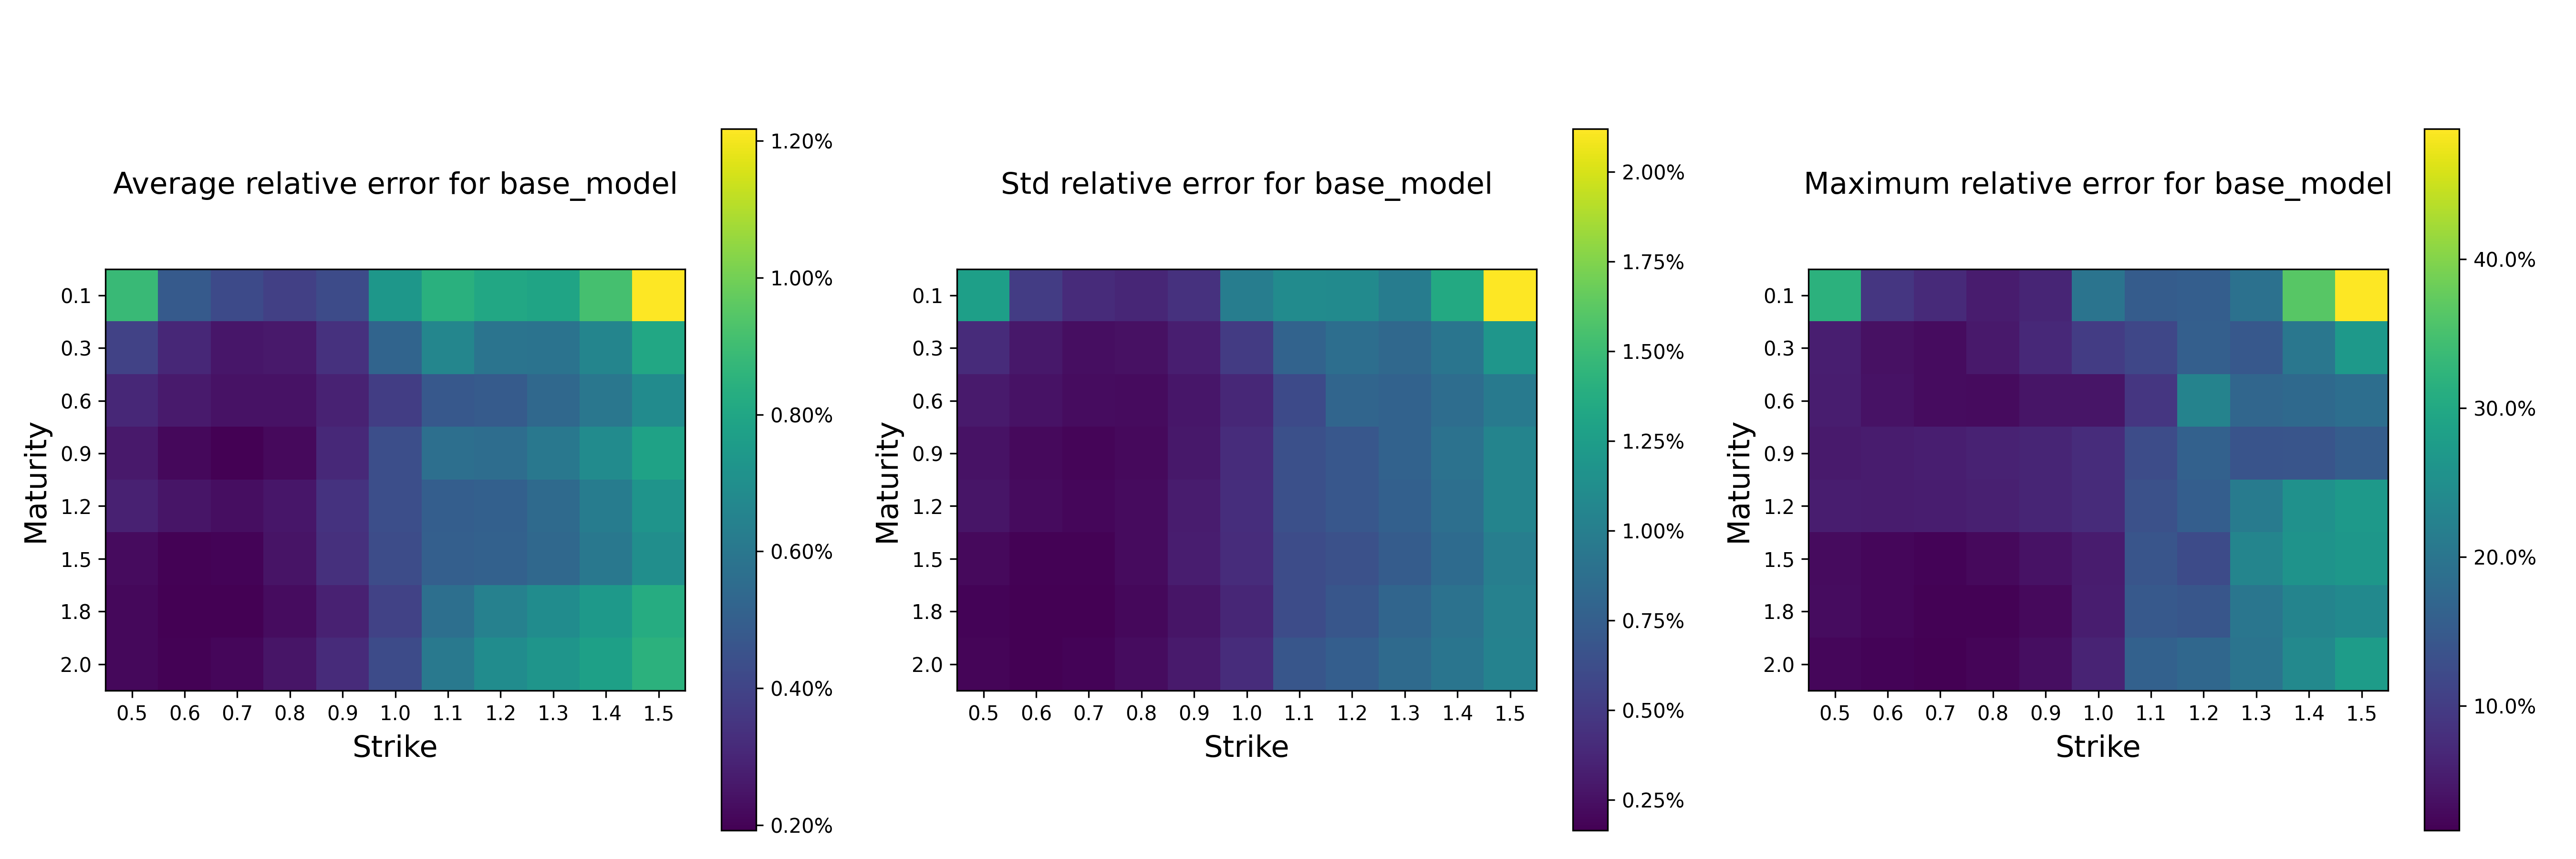
\includegraphics[width=\linewidth]{../data/rBergomiTermStructureNNErrors_Model_base_model_1.png}
  \caption{Relative errors for the baseline model, from Horvath, Muguruza and Mehdi (\cite{HMM19}), with 4 Layers.}
  \label{fig:base_model}
\end{figure}

\begin{figure}[h!]
  \centering
  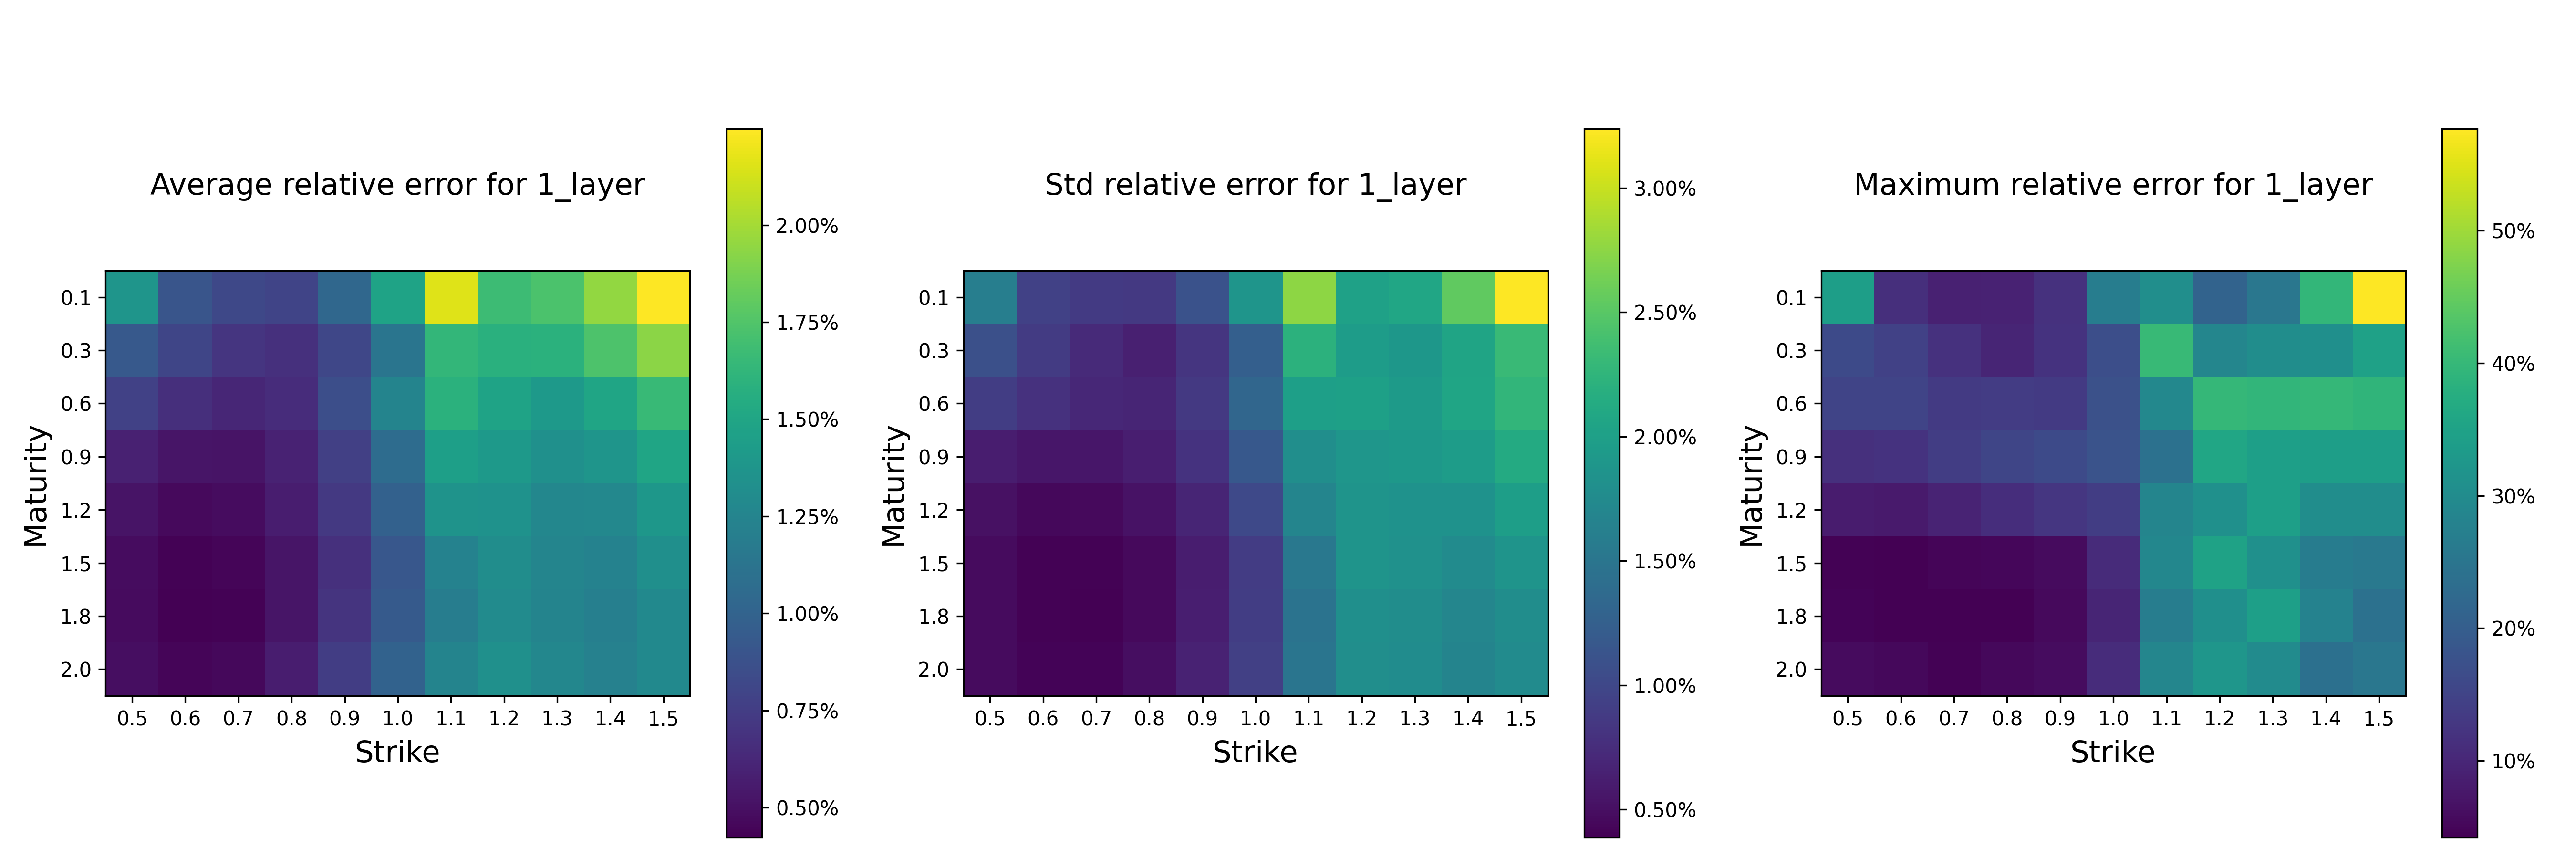
\includegraphics[width=\linewidth]{../data/rBergomiTermStructureNNErrors_Model_1_layer_5.png}
  \caption{Relative errors for the 1 layer configuration.}
  \label{fig:1_layer}
\end{figure}

\begin{figure}[h!]
  \centering
  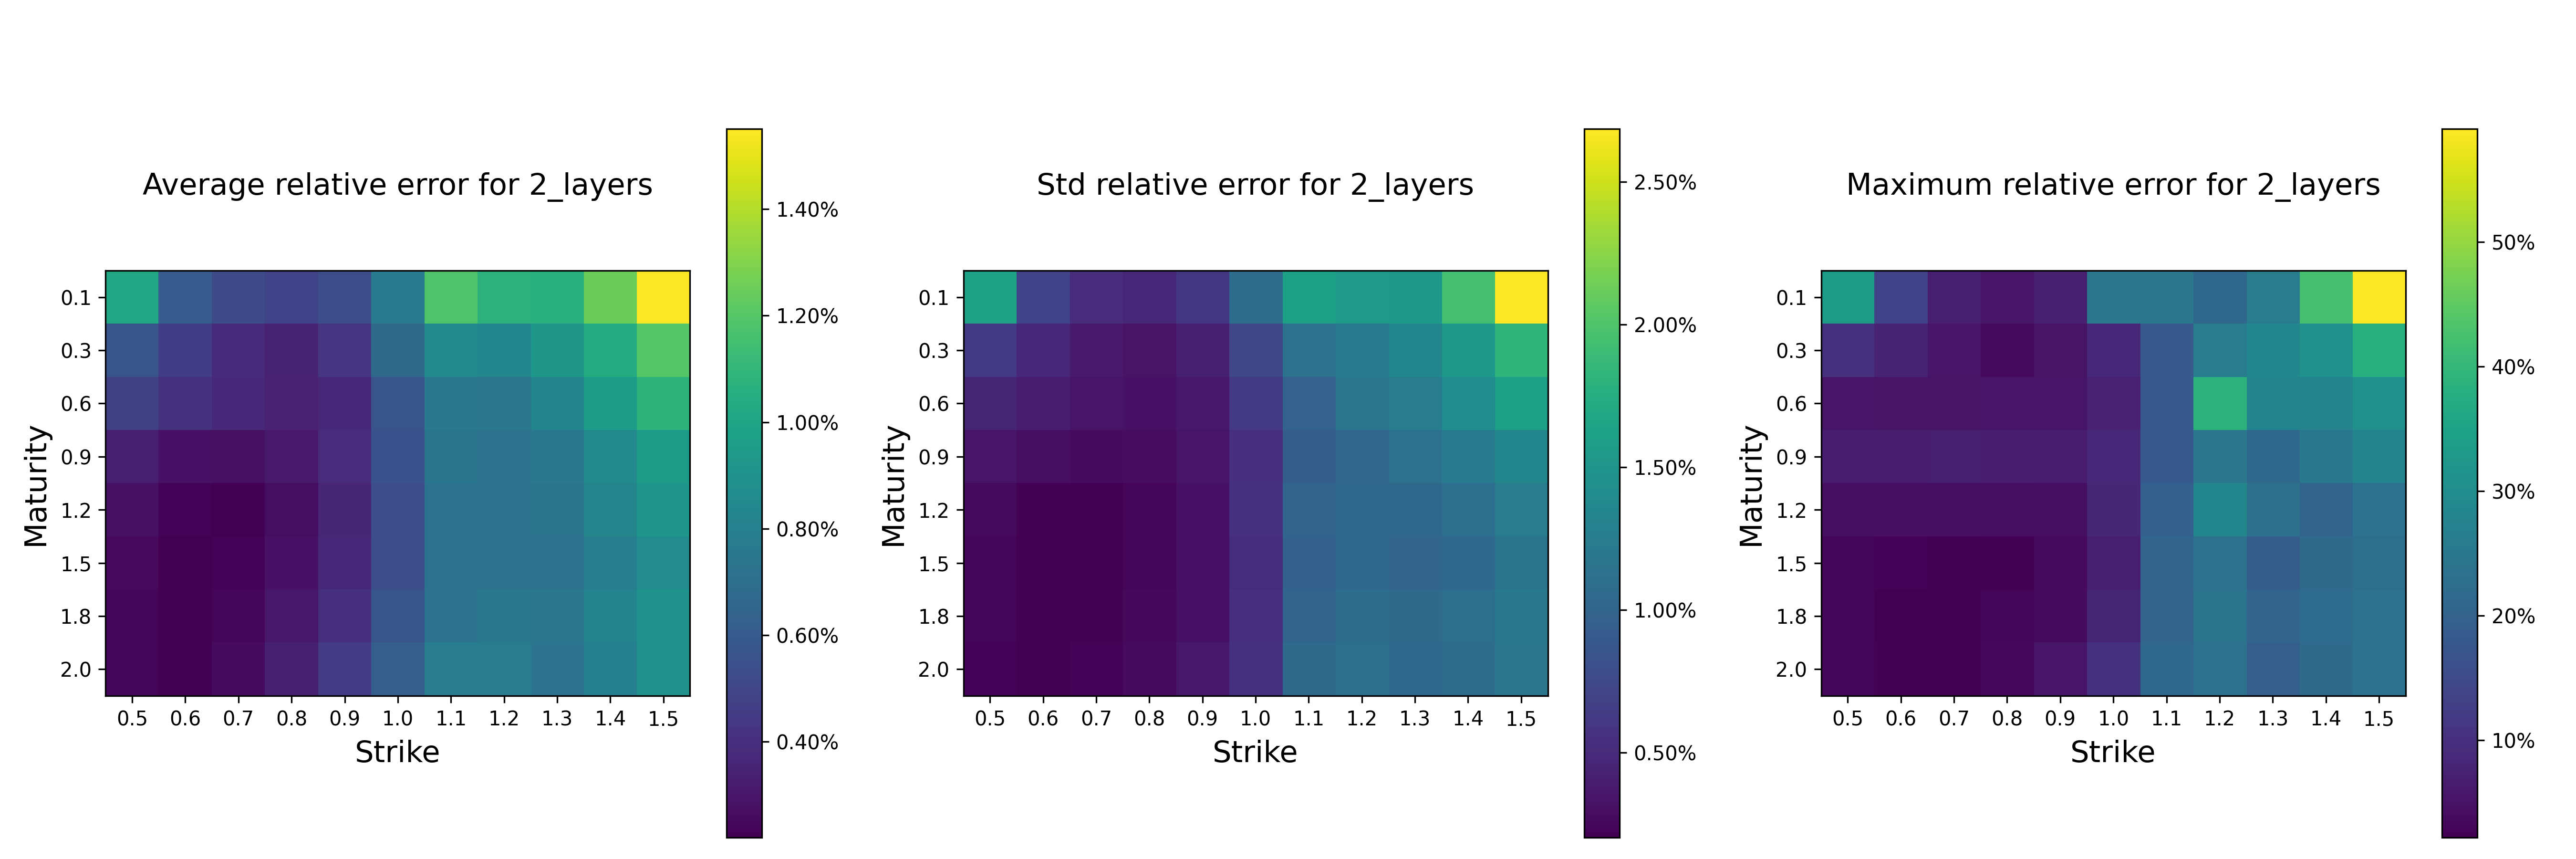
\includegraphics[width=\linewidth]{../data/rBergomiTermStructureNNErrors_Model_2_layers_6.png}
  \caption{Relative errors for the 2 layer configuration.}
  \label{fig:2_layers}
\end{figure}

\begin{figure}[h!]
  \centering
  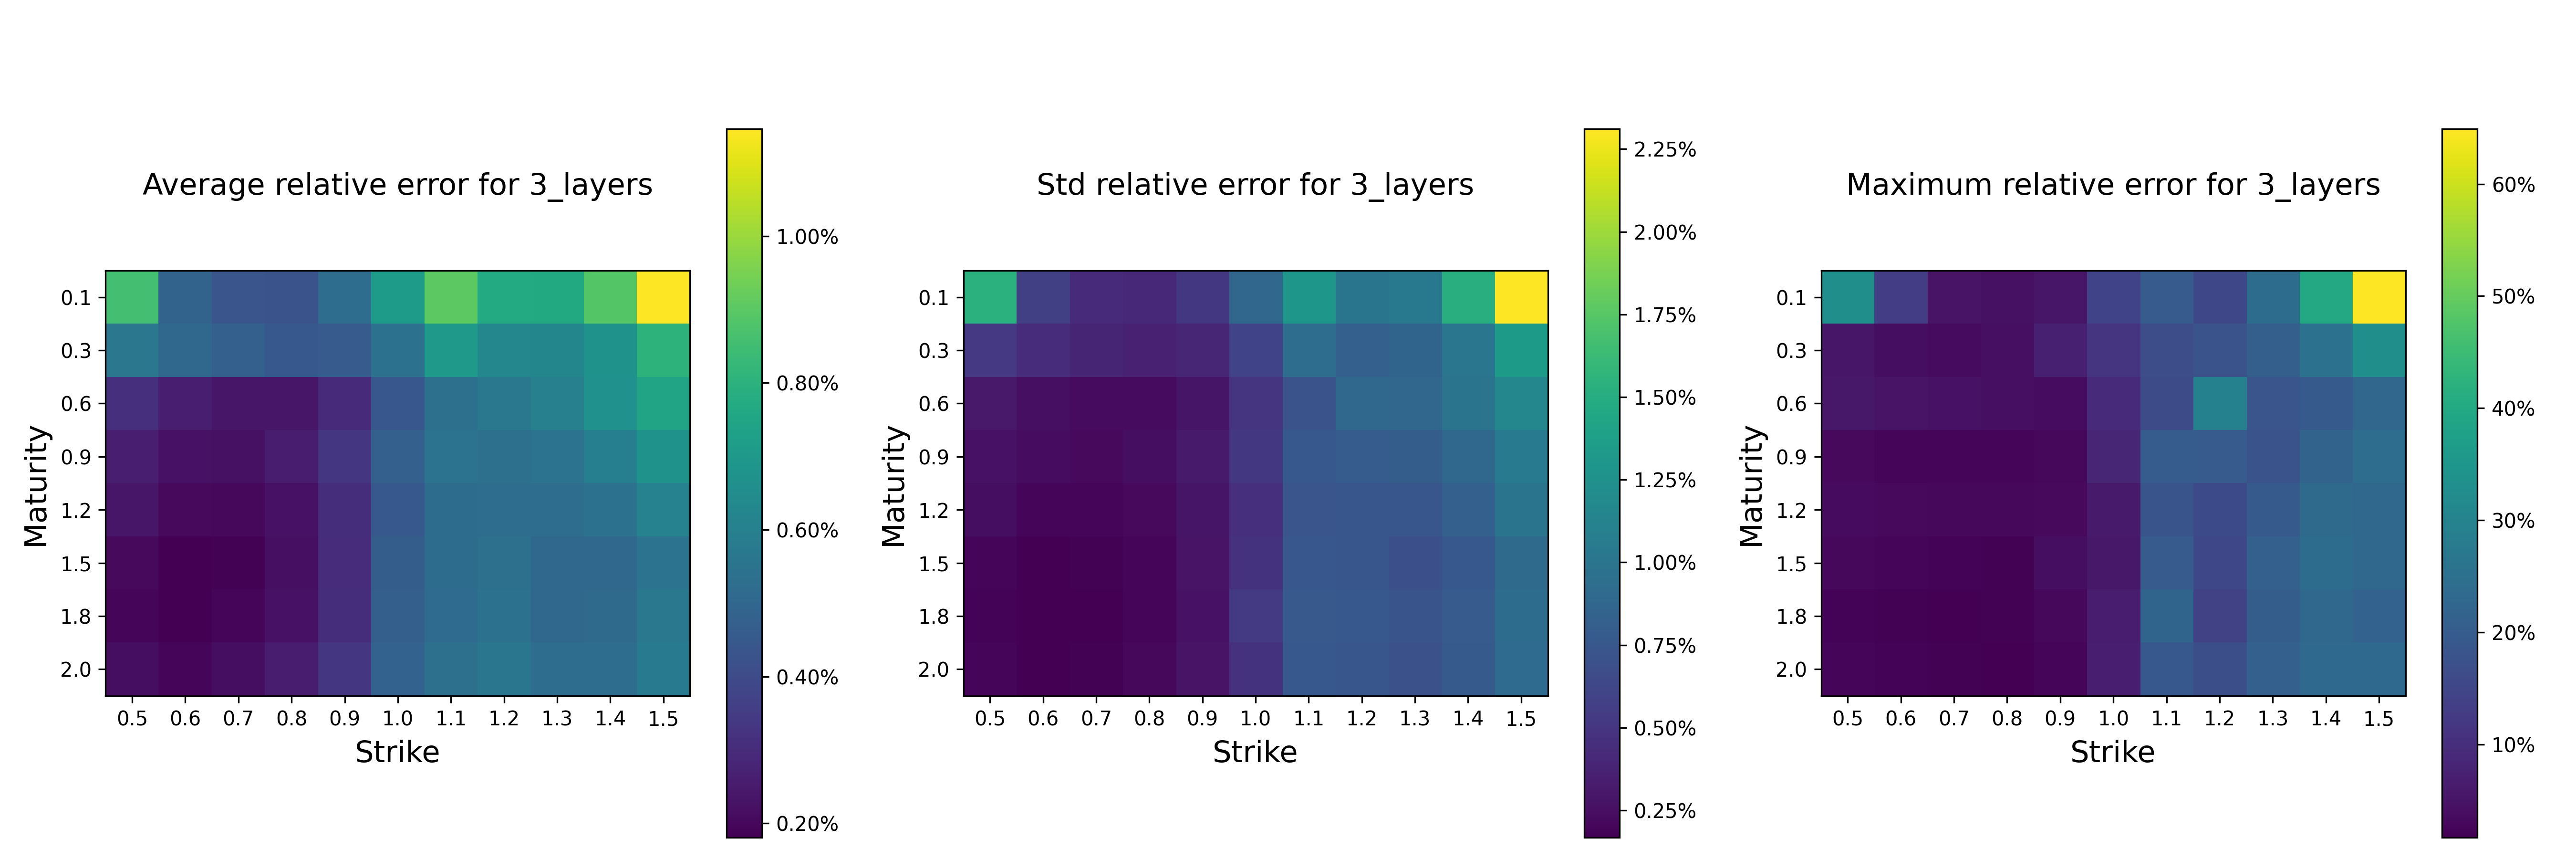
\includegraphics[width=\linewidth]{../data/rBergomiTermStructureNNErrors_Model_3_layers_7.png}
  \caption{Relative errors for the 3 layer configuration.}
  \label{fig:3_layers}
\end{figure}

\begin{figure}[h!]
  \centering
  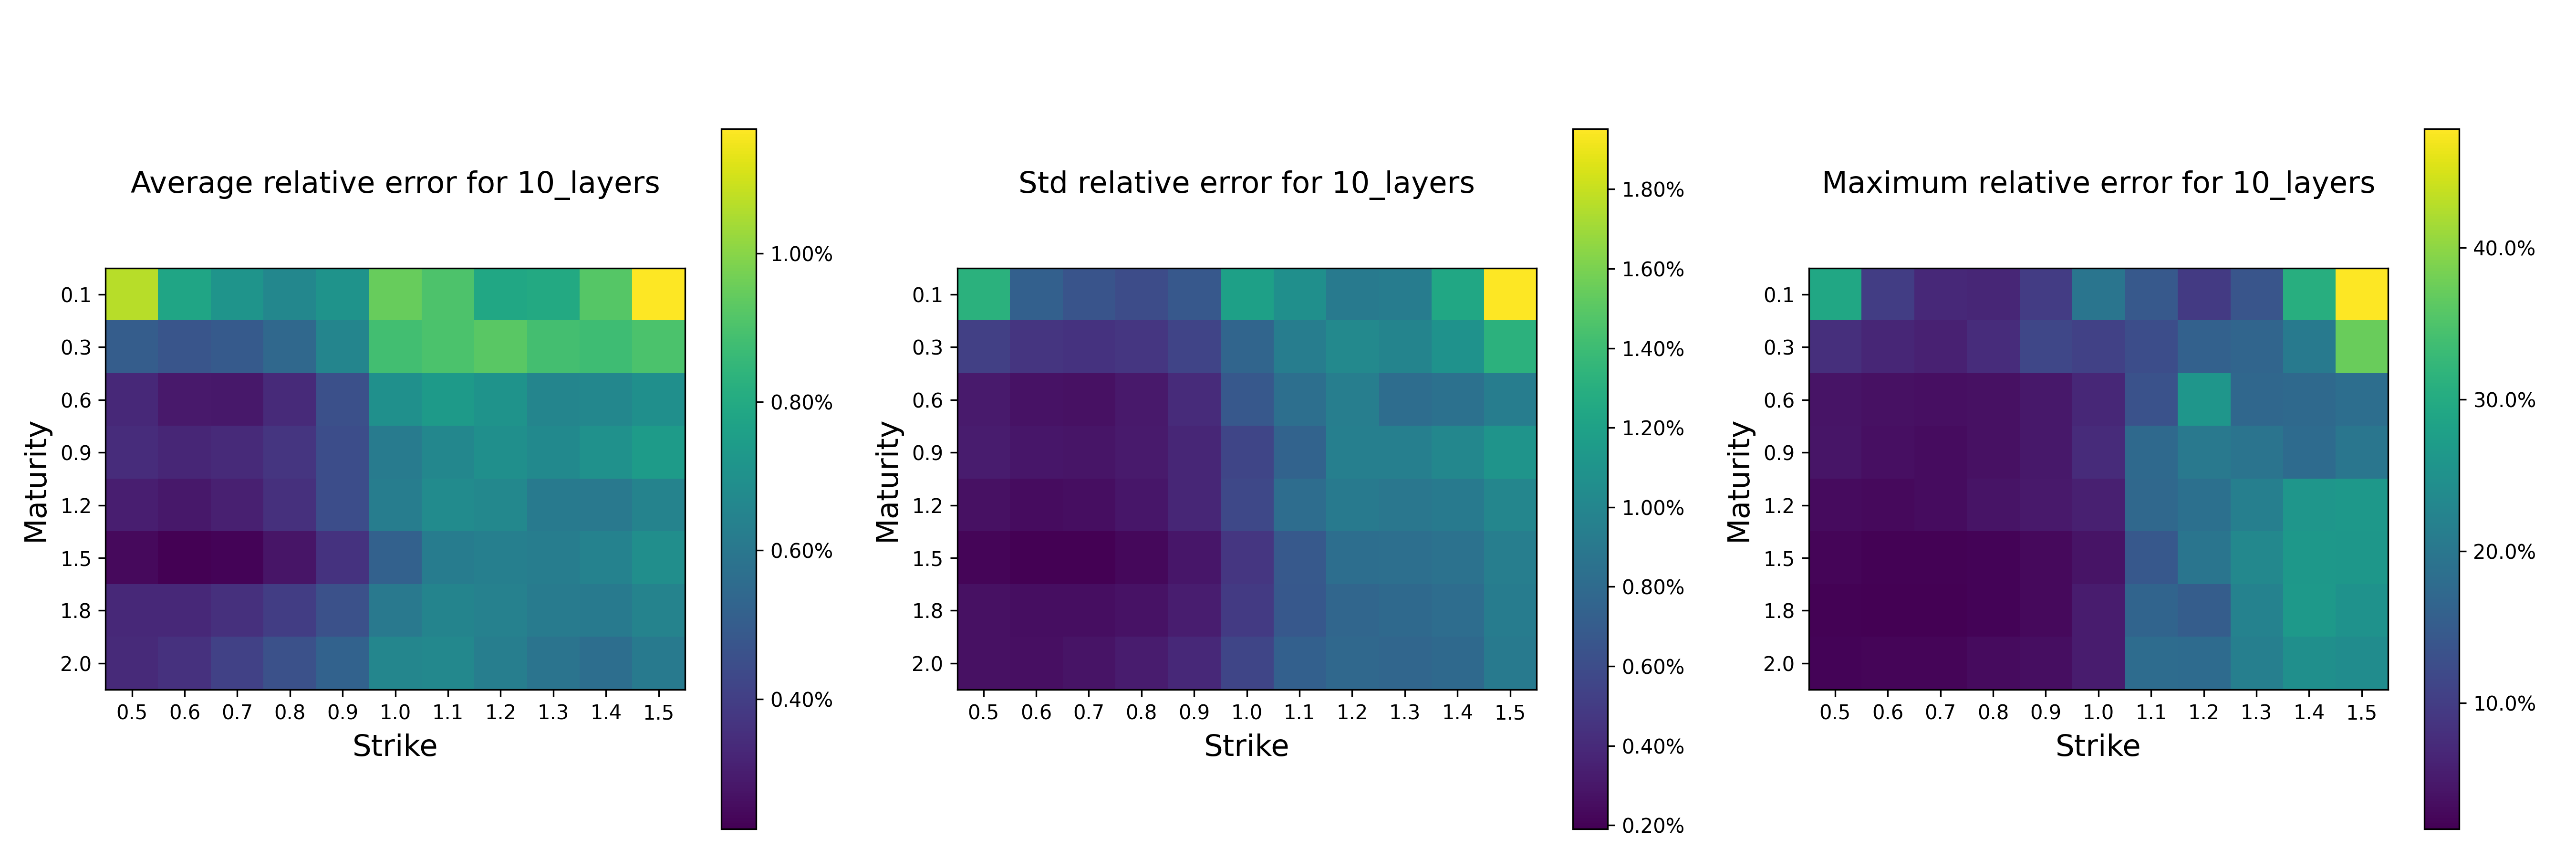
\includegraphics[width=\linewidth]{../data/rBergomiTermStructureNNErrors_Model_10_layers_2.png}
  \caption{Relative errors for the 10 layer configuration.}
  \label{fig:10_layers}
\end{figure}

\begin{figure}[h!]
  \centering
  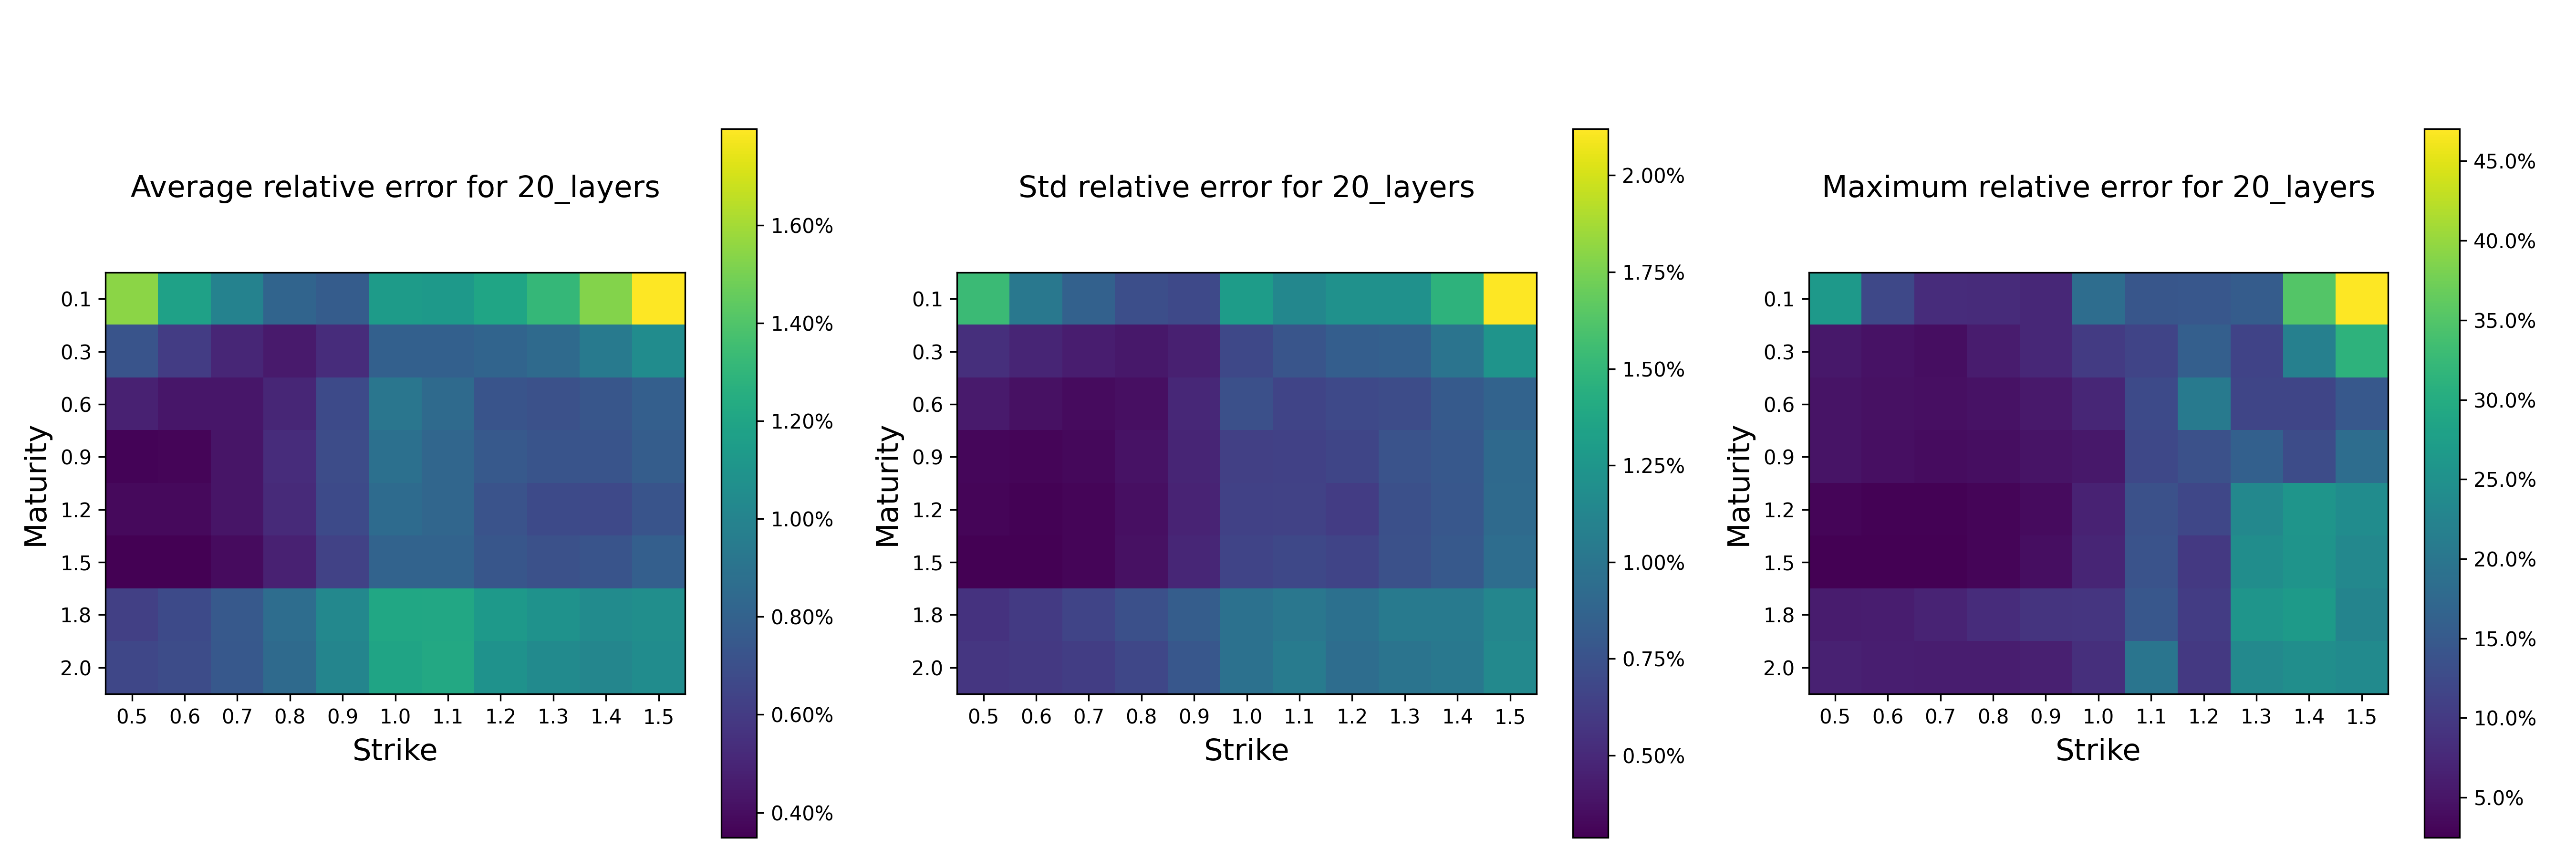
\includegraphics[width=\linewidth]{../data/rBergomiTermStructureNNErrors_Model_20_layers_3.png}
  \caption{Relative errors for the 20 layer configuration.}
  \label{fig:20_layers}
\end{figure}

\begin{figure}[h!]
  \centering
  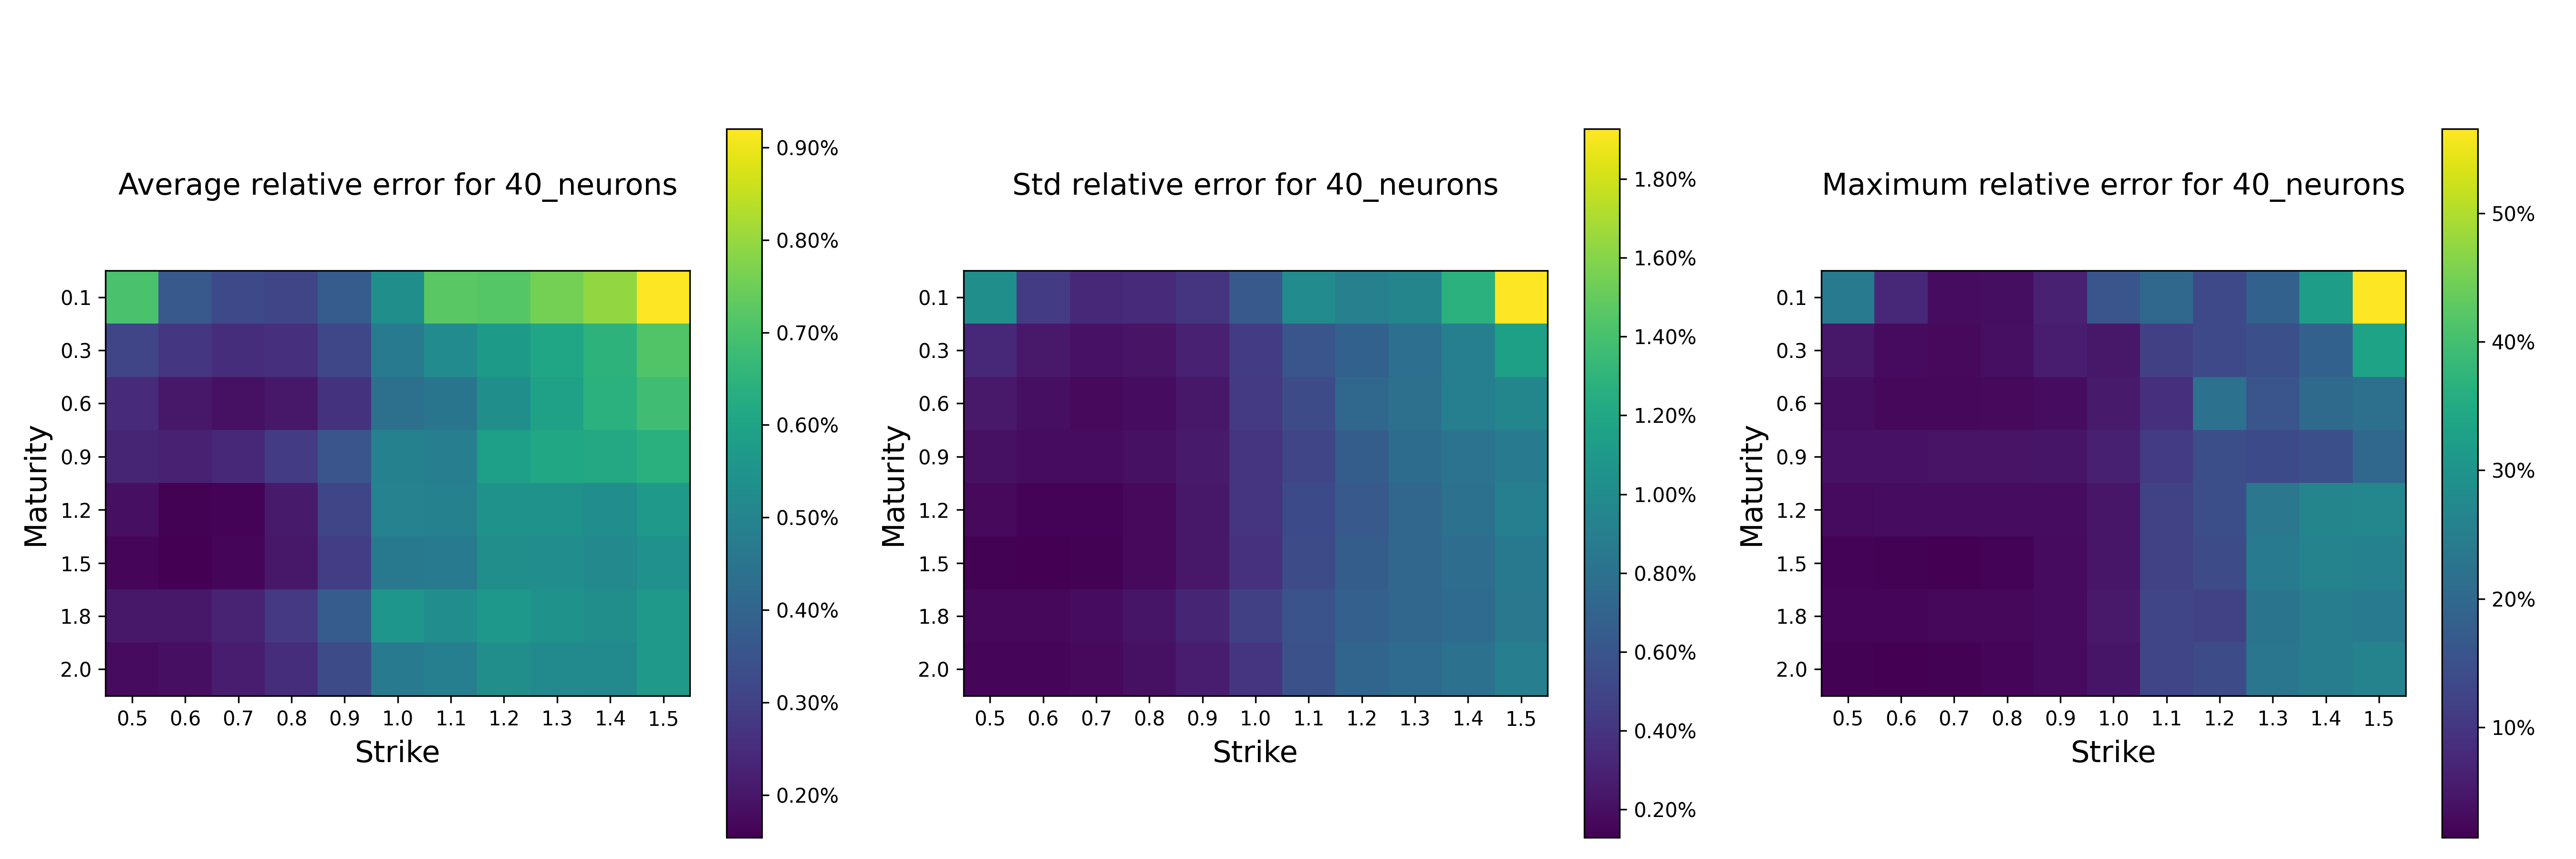
\includegraphics[width=\linewidth]{../data/rBergomiTermStructureNNErrors_Model_40_neurons_8.png}
  \caption{Relative errors for the 4 layer configuration, with 40 neurons per layer.}
  \label{fig:40_neurons}
\end{figure}

\begin{figure}[h!]
  \centering
  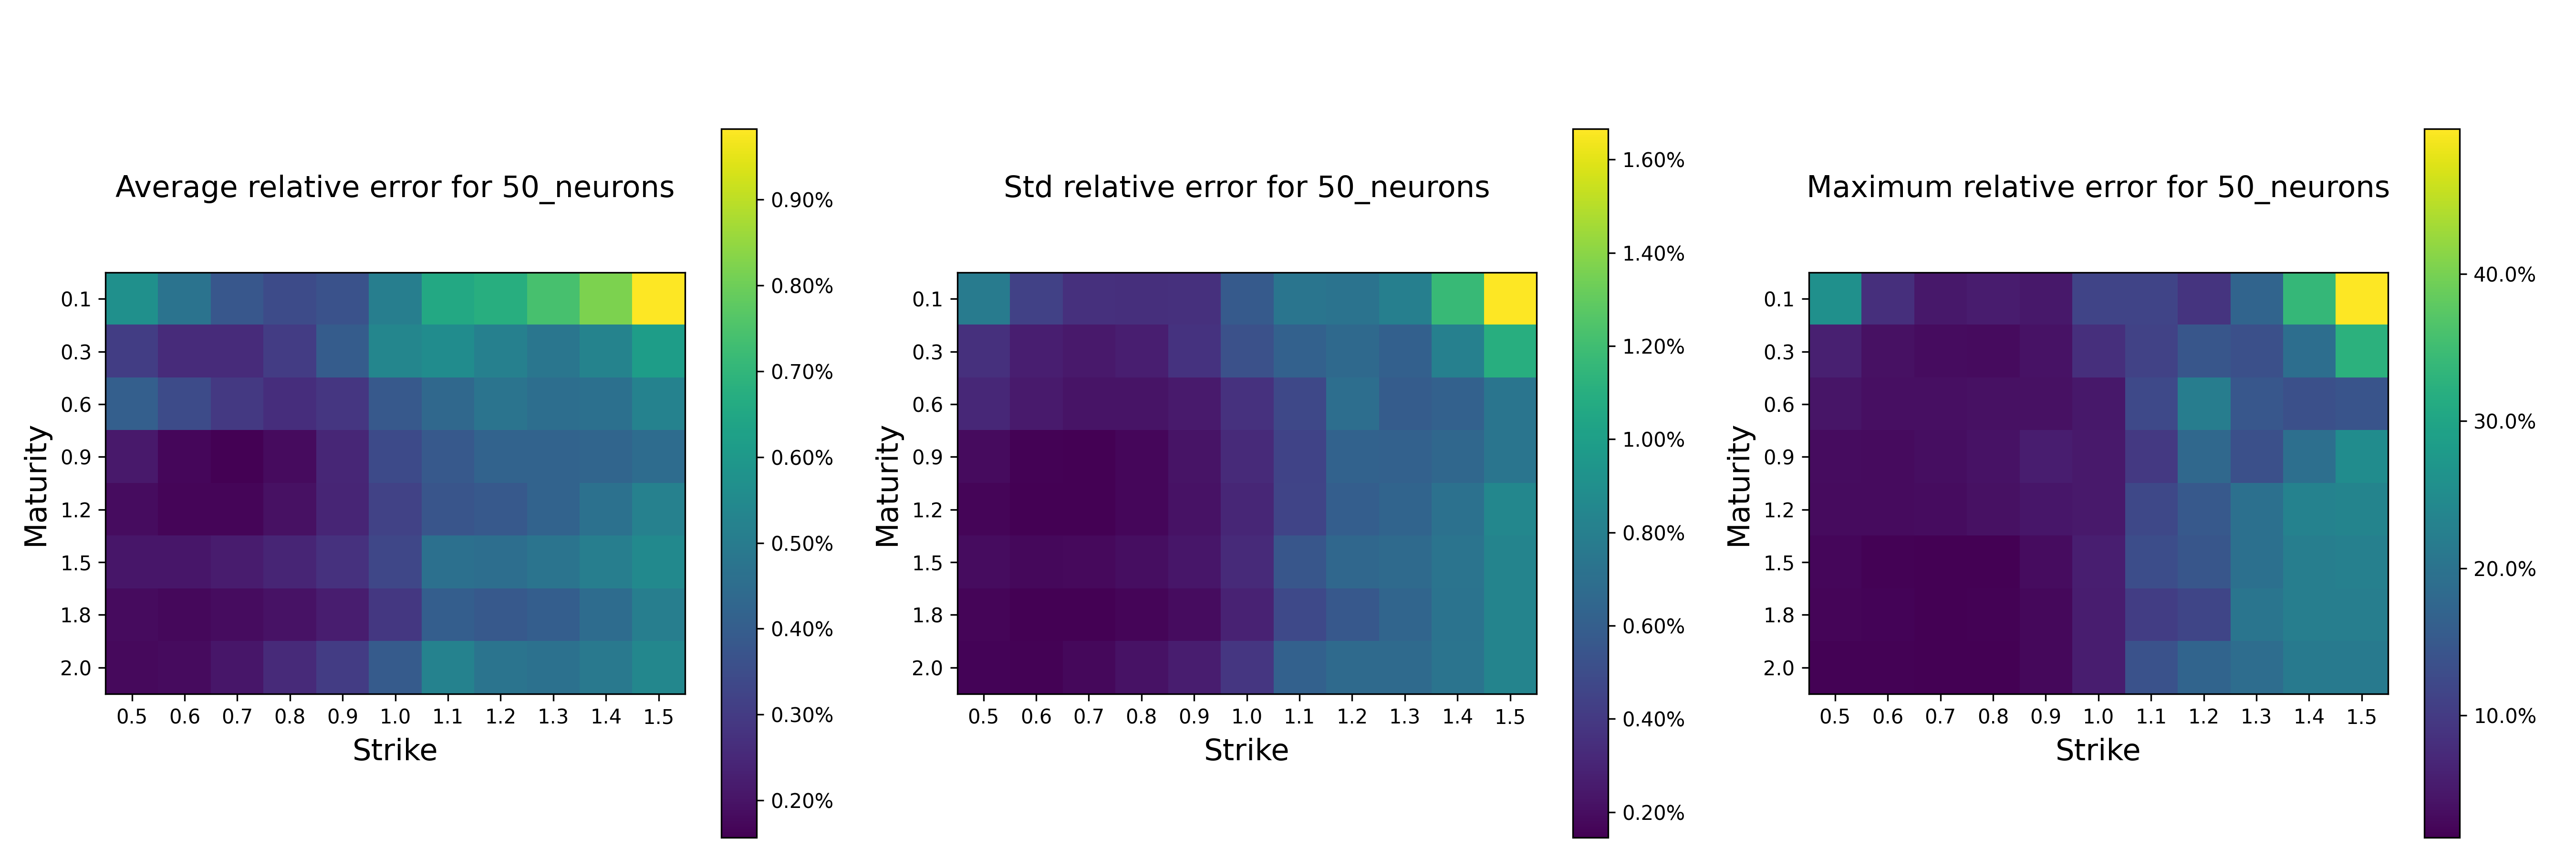
\includegraphics[width=\linewidth]{../data/rBergomiTermStructureNNErrors_Model_50_neurons_9.png}
  \caption{Relative errors for the 4 layer configuration, with 50 neurons per layer.}
  \label{fig:50_neurons}
\end{figure}

\begin{figure}[h!]
  \centering
  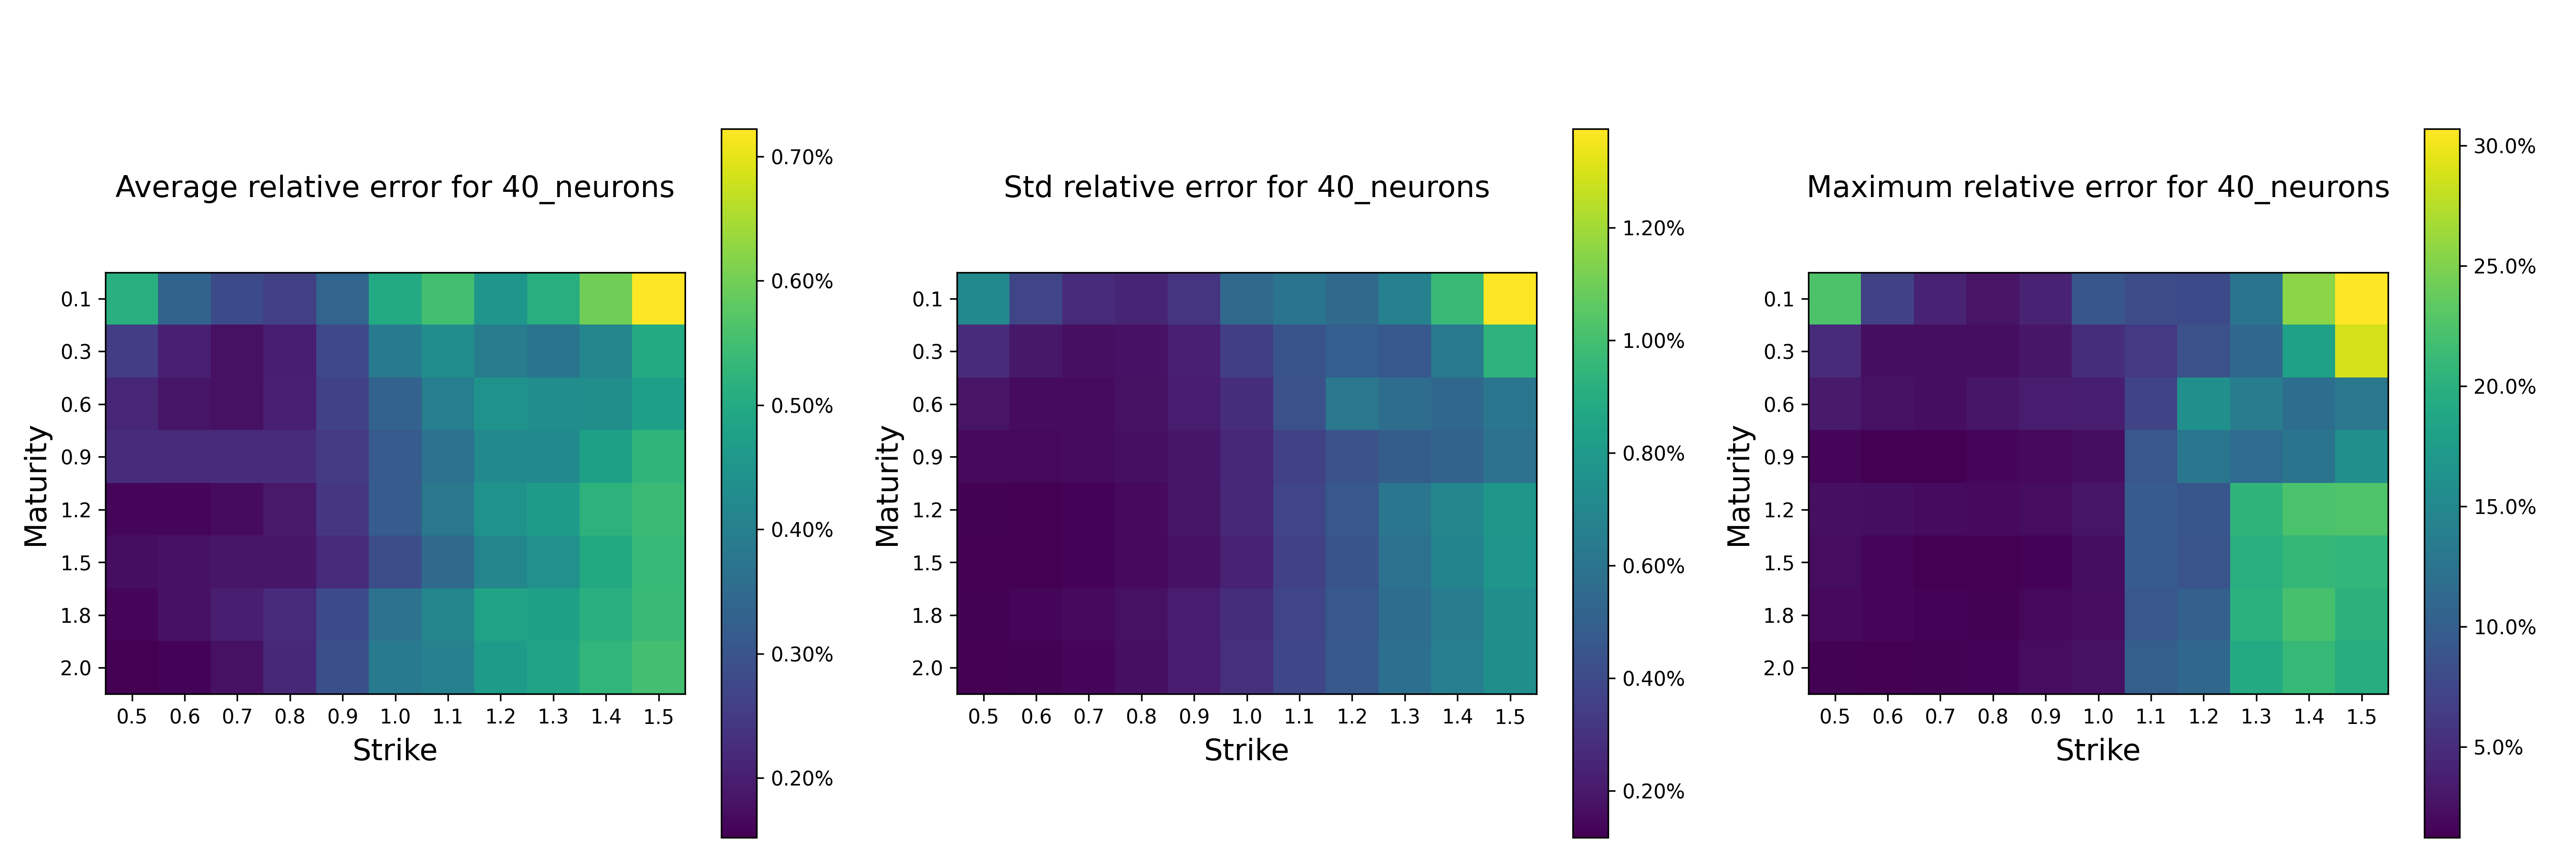
\includegraphics[width=\linewidth]{../data/rBergomiTermStructureNNErrors_Model_40_neurons_10.png}
  \caption{Relative errors for the 4 layer configuration, with 60 neurons per layer.}
  \label{fig:60_neurons}
\end{figure}

\begin{figure}[h!]
  \centering
  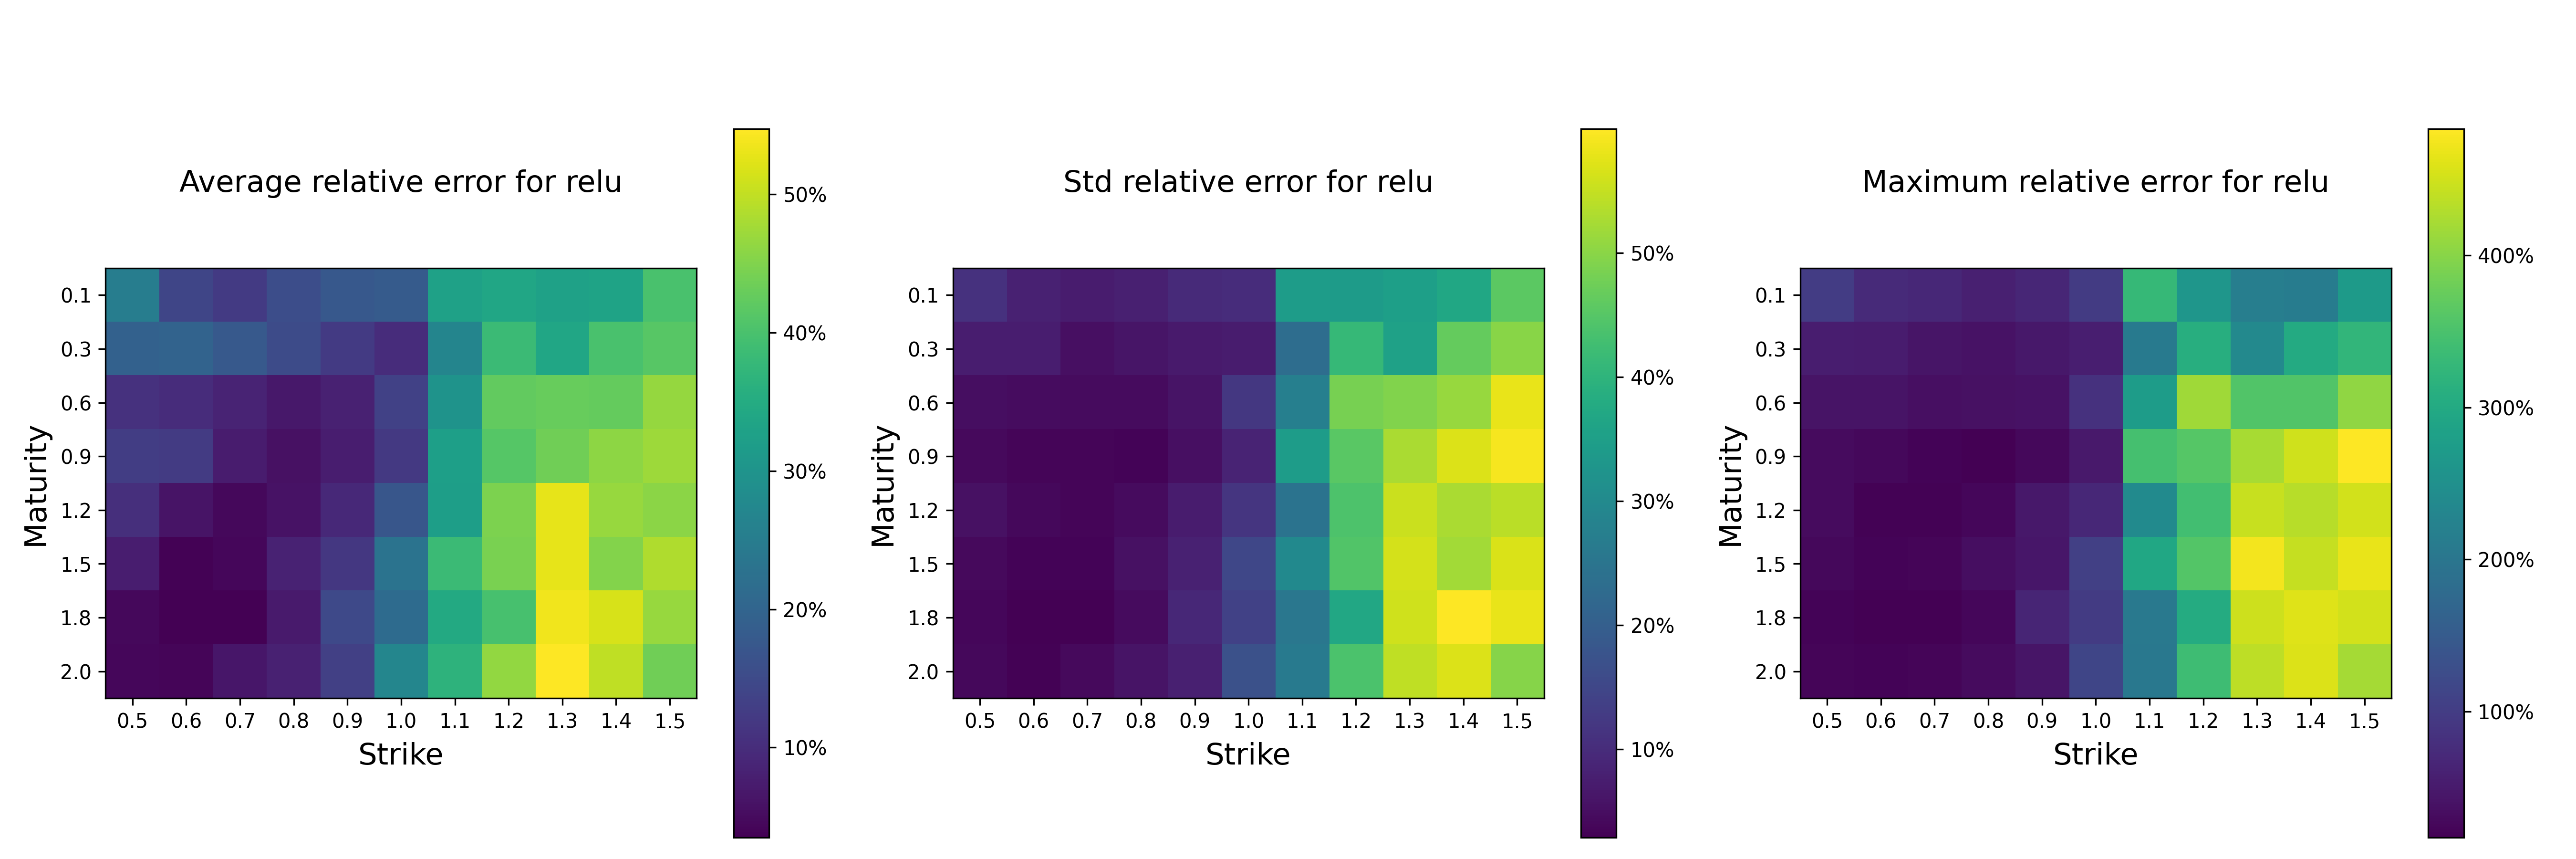
\includegraphics[width=\linewidth]{../data/rBergomiTermStructureNNErrors_Model_relu_4.png}
  \caption{Relative errors for the 4 layer configuration, with ReLu activation function.}
  \label{fig:relu}
\end{figure}

Besides these figures, we computed three key statistics for each model:
the average relative error across all strikes and maturities,
the standard deviation of the relative error across all strikes and maturities,
and the average maximum relative error across all strikes and maturities.
These statistics are summarized in Table \ref{tab:model_performance}.
\begin{table}[h!]
  \centering
  \begin{tabular}{|c|c|c|c|}
    \hline
    & \begin{tabular}[c]{@{}c@{}}Avg. Rel. Error\\ (\%)\end{tabular} & \begin{tabular}[c]{@{}c@{}}Std. Dev. Rel. Error\\ (\%)\end{tabular} & \begin{tabular}[c]{@{}c@{}}Avg. Max Rel. Error\\ (\%)\end{tabular} \\ \hline
    Base Model & 0.48\% & 0.58\% & 11.95\% \\ \hline
    1 Layer & 1.06\% & 1.29\% & 20.52\% \\ \hline
    2 Layers & 0.62\% & 0.79\% & 15.08\%\\ \hline
    3 Layers & 0.47\% & 0.61\% & 12.98\%\\ \hline
    10 Layers & 0.58\% & 0.66\% & 12.50\% \\ \hline
    20 Layers & 0.80\% & 0.74\% & 12.12\% \\ \hline
    40 Neurons & 0.43\% & 0.52\% & 11.38\% \\ \hline
    50 Neurons & 0.38\% & 0.47\% & 10.80\%\\ \hline
    60 Neurons & 0.35\%& 0.38\% & 8.54\%\\ \hline
    ReLu & 25.26\% & 24.10\% & 186.32\%\\ \hline
  \end{tabular}
  \caption{Model Performance Metrics}
  \label{tab:model_performance}
\end{table}

The analysis reveals that employing the ReLU function is suboptimal (see Figure \ref{fig:relu}).
This observation aligns with the universal approximation theorem for derivatives by Hornik, Stinchcombe, and White \cite{UniversalApprox},
as the ReLU activation function does not belong to $C^l(\mathbb{R})$ for any $l>0$, in contrast to the ELU function.

Additionally, increasing the number of layers does not yield substantial improvements.
While the average maximum relative error decreases, the average relative error actually increases compared to the base model.
Notably, the base model with four layers outperforms models with fewer layers,
although the benefits beyond three layers are marginal.
The performance gains from increasing layers from one to two are significantly greater than those from increasing from two to three,
indicating diminishing returns.

Increasing the number of neurons per layer demonstrates tangible benefits;
however, these benefits also exhibit diminishing returns.
Specifically, increasing beyond 60 neurons (mislabelled as 40 neurons in Figure \ref{fig:60_neurons})
does not result in substantial further improvements.

Furthermore, the increase in neurons leads to a corresponding increase in calibration time,
making excessive neuron counts less desirable, particularly in contexts such as fixed income desks where calibration time is critical.

Calibration times for ten different models were plotted, confirming the expected trend:
a higher number of layers or neurons increases calibration time.
For instance, the model with 20 layers required up to ten times longer to calibrate than the base model.
In comparison, increasing the number of neurons from 30 to 60 resulted in a minor increase in calibration time,
less than one millisecond longer when using the Levenberg-Marquardt algorithm, which consistently proved to be the fastest.

Comprehensive results, including relative errors for Levenberg-Marquardt optimal parameters,
are documented in the accompanying Jupyter notebook. These details were omitted here due to the lack of significant new information.

Further experiments, such as varying the number of neurons between the layers, or trying out different learning rates, is left to future research.
Overall, we confirmed that the models introduced in \cite{HMM19} can provide a great fit and allow to calibrate
the rough Bergomi model with piecewise constant forward variance curve quickly and accurately.

\appendix
\newpage
\begin{thebibliography}{99}
\bibitem{AlosLeon}E. Al\`os, J. Le\'on and J. Vives. 
On the short-time behavior of the implied volatility for jump-diffusion models with stochastic volatility. 
\textit{Finance and Stochastics}, {\tt 11}(4), 571-589, 2007.

\bibitem{BFGMS17}C.~Bayer, P.~Friz, P.~Gassiat, J.~Martin and B.~Stemper.
A regularity structure for rough volatility. 
\href{https://arxiv.org/abs/1710.07481}{arXiv:1710.07481}, 2017.

\bibitem{BFG15}C.~Bayer, P.~Friz  and J.~Gatheral.
Pricing under rough volatility. 
\textit{Quantitative Finance}, {\tt 16}(6): 1-18, 2016.

\bibitem{BFGHS}C.~Bayer, P. Friz, A. Gulisashvili, B. Horvath and B. Stemper.
Short-time near the money skew in rough fractional stochastic volatility models.
\href{https://arxiv.org/abs/1703.05132}{arXiv:1703.05132}, 2017.

\bibitem{BHMST19}C.~Bayer, B. Horvath, A. Muguruza, B. Stemper and M. Tomas.
On deep calibration of (rough) stochastic volatility models.
\href{https://arxiv.org/abs/1908.08806}{arXiv:1908.08806}, 2019.

\bibitem{BergomiBook}L.~Bergomi. Stochastic Volatility Modeling.
Chapman \& Hall/CRC financial mathematical series.  \textit{Chapman \& Hall/CRC}, 2015.

\bibitem{CulcinDas17}R. Culkin and S. R. Das 
Machine Learning in Finance: The Case of Deep Learning for Option Pricing. 
\textit{Journal of Investment Management}, \href{https:srdas.github.io/Papers/BlackScholesNN.pdf}{github:BlackScholesNN} 2017.

\bibitem{MadanSchoutens} J.~De Spiegeleer, D.~Madan, S.~Reyners and W.~Schoutens. Machine learning for quantitative finance:
Fast derivative pricing, hedging and fitting. \href{https://papers.ssrn.com/sol3/papers.cfm?abstract_id=3191050}{SSRN:3191050}, 2018.

\bibitem{HestonConvolutional} G.~Dimitroff, D.~R\"oder and C.~P. Fries. Volatility model calibration with convolutional neural networks. \textit{Preprint}, \href{https://papers.ssrn.com/sol3/papers.cfm?abstract_id=3252432}{SSRN:3252432}, 2018.

\bibitem{FZ17} M.~Forde, H.~Zhang. Asymptotics for Rough Stochastic Volatility

\bibitem{FG18} R.~Ferguson and A. D.~Green. Deeply learning derivatives.
  Preprint \href{https://arxiv.org/abs/1809.02233}{arXiv:1809.02233}, 2018.

\bibitem{Fukasawa}M. Fukasawa.
Asymptotic analysis for stochastic volatility: martingale expansion.
\textit{Finance and Stochastics}, {\tt 15}: 635-654, 2011.

\bibitem{Hagan1}P. Hagan, D. Kumar, A. Lesniewski, and D. Woodward. Managing smile risk. \textit{Wilmott Magazine}, {\tt September issue: 84-108}, 2002.

\bibitem{Hes93}S.L.~Heston. A closed-form solution for options with stochastic
  volatility with applications to bond and currency options, \textit{The Review of Financial Studies} 6(2):327--343, 1993.

\bibitem{Hernandez}A.~Hernandez. Model calibration with neural networks. \textit{Risk}, 2017.    

\bibitem{UniversalApprox}K. Hornik, M. Stinchcombe, and H. White. 
Multilayer feedforward networks are universal approximators. 
\textit{Neural Networks}, {\tt 2}(5):359-366, 1989.

\bibitem{HJM17}B.~Horvath, A.~Jacquier and A.~Muguruza.
Functional central limit theorems for rough volatility.
\href{https://arxiv.org/abs/1711.03078}{arXiv:1711.03078}, 2017.

\bibitem{HMM19}B.~Horvath,  A.~Muguruza and T.~Mehdi.
Deep learning volatility: a deep neural network perspective on pricing and calibration in (rough) volatility models
\textit{Quantitative Finance} 21(1), {\tt p. 11-27}, 2020.

\bibitem{Hutchison94}
J. M. Hutchinson, A. W. Lo and T. Poggio.
A Nonparametric Approach to Pricing and Hedging Derivative Securities Via Learning Networks.
\textit{The Journal of Finance}, {\tt 49}(3) 851-889. \textit{Papers and Proceedings Fifty-Fourth Annual Meeting of the American Finance Association, Boston, Massachusetts}, 1994.

\bibitem{KBAdam} D.P.~Kingman and J.~Ba, Adam: A Method for Stochastic Optimization. \textit{Conference paper}, 3rd International Conference for Learning Representations, 2015.

\bibitem{Levenberg} K.~Levenberg. A Method for the Solution of Certain Non-Linear Problems in Least Squares. \textit{Quarterly of Applied Mathematics}. 2: pp. 164-168, 1944.
\bibitem{Marquardt} D.~Marquardt. An Algorithm for Least-Squares Estimation of Nonlinear Parameters. \textit{SIAM Journal on Applied Mathematics}. 11 (2): pp. 431-441,1963.`

\bibitem{Ludkovski} M. Ludkovski.
Statistical Machine Learning for Quantitative Finance.
\textit{Annual review of statistics and its applications}, {\tt 10}, pp. 271-295, 2023.

\bibitem{McGhee}W.~A.~McGhee. An artificial neural network representation of the SABR stochastic volatility model. \textit{Preprint}, \href{https://ssrn.com/abstract=3288882}{SSRN:3288882}, 2018.

\bibitem{MP18} R.~McCrickerd, M.~Pakkanen, Turbocharging Monte Carlo pricing for the rough Bergomi model, \textit{Quantitative Finance} 18(11):1877-1886, 2018.

\bibitem{NelderMead} J. A. Nelder, R. Mead, A simplex method for function minimization.
\textit{Computer Journal}, {\tt 7}, pp. 308-313, 1965.

\bibitem{Stone}H. Stone. Calibrating rough volatility models: a convolutional neural network approach. \textit{Preprint}, \href{https://arxiv.org/pdf/1812.05315.pdf}{arXiv:1812.05315}, 2018.
\end{thebibliography}
\end{document}
